% ****************************************************************************************** % Dissertation template and document class for Princeton University
% Author  : Jeffrey Scott Dwoskin <jdwoskin@princeton.edu>
% Adapted from: http://www.math.princeton.edu/graduate/tex/puthesis.html
% ****************************************************************************************** %

%\includeonly{ch-intro/chapter-intro}
%\includeonly{ch-zfLandscape/chapter-zfLandscape}
%\includeonly{ch-jointInference/chapter-jointInference}
%\includeonly{ch-interfaceMapping/chapter-interfaceMapping}
%\includeonly{ch-appendicies/suppl-meths}
%\includeonly{ch-appendicies/suppl-figs-zf}
%\includeonly{ch-appendicies/suppl-figs-jointInference}
%\includeonly{ch-conclusion/chapter-conclusion}

%%% For print copies
%% set 'singlespace' option to set entire thesis to single space, and define "\printmode" to remove all hyperlinks for printed copies of the thesis. Delete all output files before changing this mode -- it will turn hyperref package on and off
%\documentclass[12pt,lot, lof, singlespace]{puthesis}
%\newcommand{\printmode}{}

%%% For the electronic copy, use doublespacing, define "\proquestmode" to use outlined links, instead of colored links. 
\documentclass[12pt,lof]{puthesis}
\newcommand{\proquestmode}{}
% I prefer proquestmode to be off for electronic copies for normal use, since the colored links are less distracting. However when printed in black and white, the colored links are difficult to read. 

%%% For early drafts without some of the frontmatter
% Also see the "ifodd" command below to disable more frontmatter
%\documentclass[12pt]{puthesis}

\usepackage{amssymb}
\usepackage{amsthm}
\usepackage{mathtools}
\usepackage{pdfpages}
\usepackage{bm}
\usepackage{mathptmx}
\usepackage{subcaption}
\usepackage{dirtytalk}
%\usepackage[T1]{fontenc}
%\usepackage[scaled]{helvet}
%\usepackage{times}
%\renewcommand*\familydefault{\sfdefault}

\newtheorem{definition}{Definition}
\newtheorem{lemma}{Lemma}
\newtheorem*{lemma*}{}
\newtheorem{theorem}{Theorem}
\newtheorem{corollary}{Corollary}
\newtheorem{claim}{Claim}

% Bibliography
\usepackage{natbib}


%%%%%%%%%%%%%%%%%%%%%%%%%%%%%%%%%%%%%%%%%%%%%%%%%%%%%%%%%%%%%\
%%%% Author & title page info

\title{Consumer protection on the Web with longitudinal data collection and analysis}

\submitted{April 2022}  % degree conferral date (January, April, June, September, or November)
\copyrightyear{2022}  % year in which the copyright is secured by publication of the dissertation.
\author{Ryan Amos}
\adviser{Professors Edward Felten and Prateek Mittal}  %replace with the full name of your adviser
%\departmentprefix{Program in}  % defaults to "Department of", but programs need to change this.
\department{Computer Science}

%%%%%%%%%%%%%%%%%%%%%%%%%%%%%%%%%%%%%%%%%%%%%%%%%%%%%%%%%%%%%\
%%%% Tweak float placements
% From: http://mintaka.sdsu.edu/GF/bibliog/latex/floats.html "Controlling LaTeX Floats"
% and based on: http://www.tex.ac.uk/cgi-bin/texfaq2html?label=floats
% LaTeX defaults listed at: http://people.cs.uu.nl/piet/floats/node1.html

% Alter some LaTeX defaults for better treatment of figures:
    % See p.105 of "TeX Unbound" for suggested values.
    % See pp. 199-200 of Lamport's "LaTeX" book for details.
    %   General parameters, for ALL pages:
    \renewcommand{\topfraction}{0.85}	% max fraction of floats at top
    \renewcommand{\bottomfraction}{0.6}	% max fraction of floats at bottom
    %   Parameters for TEXT pages (not float pages):
    \setcounter{topnumber}{2}
    \setcounter{bottomnumber}{2}
    \setcounter{totalnumber}{4}     % 2 may work better
    \setcounter{dbltopnumber}{2}    % for 2-column pages
    \renewcommand{\dbltopfraction}{0.66}	% fit big float above 2-col. text
    \renewcommand{\textfraction}{0.15}	% allow minimal text w. figs
    %   Parameters for FLOAT pages (not text pages):
    \renewcommand{\floatpagefraction}{0.66}	% require fuller float pages
	% N.B.: floatpagefraction MUST be less than topfraction !!
    \renewcommand{\dblfloatpagefraction}{0.66}	% require fuller float pages

% The documentclass already sets parameters to make a high penalty for widows and orphans. 

%%%%%%%%%%%%%%%%%%%%%%%%%%%%%%%%%%%%%%%%%%%%%%%%%%%%%%%%%%%%%\
%%%% Use packages

%\usepackage{amsfonts}

%%% For figures
\usepackage{graphicx}
%\usepackage{subfig,rotate}

%%% for comments
\usepackage{verbatim}

%%% For tables
\usepackage{multirow}
% Longtable lets you have tables that span multiple pages.
\usepackage{longtable}

% Booktabs produces far nicer tables than the standard LaTeX tables.
%   see: http://en.wikibooks.org/wiki/LaTeX/Tables
\usepackage{booktabs}

%set parameters for longtable:
% default caption width is 4in for longtable, but wider for normal tables
\setlength{\LTcapwidth}{\textwidth}

\usepackage[font=normalsize,labelfont=bf]{caption}

%%%%%%%%%%%%%%%%%%%%%%%%%%%%%%%%%%%%%%%%%%%%%%%%%%%%%%%%%%
%%% Printed vs. online formatting
\ifdefined\printmode

% Printed copy
% url package understands urls (with proper line-breaks) without hyperlinking them
\usepackage{url}


\else

\ifdefined\proquestmode
%ProQuest copy -- http://www.princeton.edu/~mudd/thesis/Submissionguide.pdf

% ProQuest requires a double spaced version (set previously). They will take an electronic copy, so we want links in the pdf, but also copies may be printed or made into microfilm in black and white, so we want outlined links instead of colored links.
\usepackage{hyperref}
\hypersetup{bookmarksnumbered}

% copy the already-set title and author to use in the pdf properties
\makeatletter
\hypersetup{pdftitle=\@title,pdfauthor=\@author}
\makeatother

\else
% Online copy

% adds internal linked references, pdf bookmarks, etc

% turn all references and citations into hyperlinks:
%  -- not for printed copies
% -- automatically includes url package
% options:
%   colorlinks makes links by coloring the text instead of putting a rectangle around the text.
\usepackage{hyperref}
\hypersetup{colorlinks,bookmarksnumbered}

% copy the already-set title and author to use in the pdf properties
\makeatletter
\hypersetup{pdftitle=\@title,pdfauthor=\@author}
\makeatother

% make the page number rather than the text be the link for ToC entries
%\hypersetup{linktocpage}
\fi % proquest or online formatting
\fi % printed or online formatting


%%%%%%%%%%%%%%%%%%%%%%%%%%%%%%%%%%%%%%%%%%%%%%%%%%%%%%%%%%%%%\
%%%% Define commands

% Define any custom commands that you want to use.
% For example, highlight notes for future edits to the thesis
%\newcommand{\todo}[1]{\textbf{\emph{TODO:}#1}}


% create an environment that will indent text
% see: http://latex.computersci.org/Reference/ListEnvironments
% 	\raggedright makes them left aligned instead of justified
\newenvironment{indenttext}{
    \begin{list}{}{ \itemsep 0in \itemindent 0in
    \labelsep 0in \labelwidth 0in
    \listparindent 0in
    \topsep 0in \partopsep 0in \parskip 0in \parsep 0in
    \leftmargin 1em \rightmargin 0in
    \raggedright
    }
    \item
  }
  {\end{list}}

% another environment that's an indented list, with no spaces between items -- if we want multiple items/lines. Useful in tables. Use \item inside the environment.
% 	\raggedright makes them left aligned instead of justified
\newenvironment{indentlist}{
    \begin{list}{}{ \itemsep 0in \itemindent 0in
    \labelsep 0in \labelwidth 0in
    \listparindent 0in
    \topsep 0in \partopsep 0in \parskip 0in \parsep 0in
    \leftmargin 1em \rightmargin 0in
    \raggedright
    }

  }
  {\end{list}}
  
  
%Note command
\newcommand{\raNote}[1]{{\color{blue}[{{#1}}]}}



%%%%%%%%%%%%%%%%%%%%%%%%%%%%%%%%%%%%%%%%%%%%%%%%%%%%%%%%%%%%%\
%%%% Front-matter

% For early drafts, you may want to disable some of the frontmatter. Simply change this to "\ifodd 1" to do so.
\ifodd 0
% front-matter disabled while writing chapters
\renewcommand{\maketitlepage}{}
\renewcommand*{\makecopyrightpage}{}
\renewcommand*{\makeabstract}{}

% you can just skip the \acknowledgements and \dedication commands to leave out these sections.

\else


\abstract{
% Abstract can be any length, but should be max 350 words for a Dissertation for ProQuest's print indicies (150 words for a Master's Thesis) or it will be truncated for those uses.
Automated analysis of privacy policies has proved a fruitful research direction, with developments such as automated policy summarization, question answering systems, and compliance detection. Prior research has been limited to analysis of privacy policies from a single point in time or from short spans of time, as researchers did not have access to a large-scale, longitudinal, curated dataset. To address this gap, we developed a crawler that discovers, downloads, and extracts archived privacy policies from the Internet Archive’s Wayback Machine. Using the crawler and following a series of validation and quality control steps, we curated a dataset of 1,071,488 English language privacy policies, spanning over two decades and over 130,000 distinct websites. 

Our analyses of the data paint a troubling picture of the transparency and accessibility of privacy policies. By comparing the occurrence of tracking-related terminology in our dataset to prior web privacy measurements, we find that privacy policies have consistently failed to disclose the presence of common tracking technologies and third parties. We also find that over the last twenty years privacy policies have become even more difficult to read, doubling in length and increasing a full grade in the median reading level. Our data indicate that self-regulation for first-party websites has stagnated, while self-regulation for third parties has increased but is dominated by online advertising trade associations. Finally, we contribute to the literature on privacy regulation by demonstrating the historic impact of the GDPR on privacy policies.

}

\acknowledgements{
%I would like to thank...
Faculty who have advised me:
Chris Bailey-Kellogg
Sean Smith
Jason Moore
Mona Singh
Mark Zhandry
Ed Felten
Prateek Mittal
Arvind Narayanan
Jonathan Mayer
Peter Andrews


Co-authors
Gunes Acar
Sam Ginzberg
Eli Lucherini
Mihir Kshisagar
}

\dedication{To ...}

\fi  % disable frontmatter



%%%%%%%%%%%%%%%%%%%%%%%%%%%%%%%%%%%%%%%%%%%%%%%%%%%%%%%%%%%%%\
%%%% Hide some chapters

%%% If you want to produce a pdf that includes only certain chapters, specify them with includeonly, in addition to including all chapters below.
%\includeonly{ch-intro/chapter-intro}
%%% You can also specify multiple chapters.
%\includeonly{ch-intro/chapter-intro,ch-usage/chapter-usage}
%\includeonly{chap1,chap2,chap3}


%%%%%%%%%%%%%%%%%%%%%%%%%%%%%%%%%%%%%%%%%%%%%%%%%%%%%%%%%%%%%
%%%% Notes:

% Footnotes should be placed after punctuation.\footnote{place here.}
% Generally, place citations before the period~\cite{anotherauthor}.
% The proper usage for i.e., and e.g., include commas ``(e.g., option A, option B)''

%%%%%%%%%%%%%%%%%%%%%%%%%%%%%%%%%%%%%%%%%%%%%%%%%%%%%%%%%%%%%
%%%% Import chapters

\begin{document}

\makefrontmatter


% If you've disabled frontmatter, you can insert the toc manually
%\tableofcontents\clearpage

% \include lets us split up the document (and each include starts a new page):
\chapter{Introduction} \label{ch:introduction}

%\raNote{``Thesis'' sentence, which should absolutely go somewhere in here, bolded: When using web crawls to study consumer protection issues, researchers should consider repeated crawls rather than a single, monolithic crawl.}

The rise of the internet has introduced new challenges in consumer protection. Cheap and efficient data collection has introduced unique avenues for revenue generation, resulting in an amazing variety of free or low cost services at a steep cost to consumer privacy. Global marketplaces have lead to large drops in prices as online platforms reduce market friction and increase competition. When combined with a powerful capacity to amplify speech, the internet has created a strong incentive to dishonestly push narratives and opinions for one's benefit, for example posting by fake reviews. The very anonymity that protects those voices also protects the voices of those seeking to be dishonest. Consumer protection laws are crucial to defend consumers in this challenging space.

\textbf{When collecting web data to study consumer protection issues, researchers should consider repeated and longitudinal data collection rather relying than a single, monolithic crawl.} A common approach for studying consumer protection issues on the internet is to collect data from websites and analyze the data to understand the issues. For small measurements, researchers may choose to perform their data collection by hand; however for datasets numbering in the hundreds of thousands of documents or larger, this approach soon becomes infeasible and researchers turn to web crawlers, automated collection tools. Either of these approaches assumes that the web is a static place; however, as we will show in this work, this is far from true.

\section{Challenges in consumer protection}

\textbf{Consumer protection is a challenge that dates back millennia.}
Consumer protection issues likely date back to the beginning of commerce, even when face-to-face communication dominated. The story of the discovery of the Archimedes Principle could be interpreted as a consumer protection issue (if a monarch can be considered a consumer): the premise of the story is that the monarch tasked Archimedes with determining whether or not a gold crown was made of pure gold without damaging the crown~\cite{thompson2008archimedes}. This suggests that concern of deception in the marketplace is millennia old.  The standardization of weights and measures in ancient Greece and Rome can be interpreted as consumer protection rules, designed to ensure consumers recieved a fair share~\cite{smither2017roman}. Another example is the \textit{Manusmiriti} dating to around 700BCE in India, which lays out prohibitions on deceptive sales, for example of counterfeit goods or unclean food~\cite{devi2016legal}.

\textbf{Emerging technologies present new consumer protection challenges.}
In the years since, novel technologies, especially communication technologies, have introduced novel consumer protection issues. New technologies open up opportunities for those seeking revenue at the expense of consumer welfare. There are many possible reasons for this, we suggest a few possibilities: consumers aren't familiar with potential pitfalls; new technologies allow for greater scale, amplifying the marginal benefit of the smallest of gains; and that such scale may allow for diminished accountability, as alienating individual consumers has less impact. Ultimately, consumer protection issues come down to a conflict between the financial incentives of the merchant and the welfare of the consumer.

Scams are facilitated through technologies such as the postal system~\cite{uspismailfraud} and the telephone~\cite{ftcphonescams}. Improvements in banking led to the need to protect consumers against predatory or otherwise anti-consumer lending practices~\cite{eaglesham2011warning,doddfrank}. Research has shown that television programs have an influence on children's diets~\cite{morton1985television}. Most recently, the introduction of the internet has lead to a host of new consumer protection issues. Websites offer poor privacy protections while collecting large swaths of data~\cite{estrada2017online}. New types of frauds and scams have emerged~\cite{ftcscamalerts}. Access to large audiences by individuals has lead to challenges with sponsorship disclosures~\cite{ftc2021disclosures}. New methods of interacting with businesses have lead to the phenomenon of dark patterns~\cite{darkpatternsorg}.

\textbf{Consumer protection through legislation.}
Today, many jurisdictions ranging from local to national have passed consumer protection laws. In the United States, a leading national agency governing consumer protection on the internet is the Federal Trade Commission (FTC), established by the Federal Trade Commission Act of 1914~\cite{ftcact}. Many states have their own laws and entities focused on consumer protection. The FTC has highlighted a number of issues at the intersection of the internet and consumer protection including fair reviews and adequate disclosure of privacy practices~\cite{ftc20approves,ftc21notice,ftc2021disclosures,ftc-privacy-survey1998,ftc-privacy-survey2000,ftc2021canspam,ftc1997principles}.

Consumer protection law is not limited to the US and Europe. For example, Taiwan introduced a consumer protection law in 1994, although powerful industry lobbies and lack of consumer action made early enforcement challenging.~\cite{juang1997taiwan}. Nigeria implemented a federal commission to address consumer protection issues, the Federal Competition and Consumer Protection Commission; however, some academics have expressed skepticism at the decision to merge consumer protection and competition issues~\cite{tavuyanago2020interface}.

Consumer protection issues are occasionally addressed through non-profits. For example, the Better Business Bureau (BBB) is a non-profit that focuses on consumer protection through industry self-regulation. However, many have cast doubt on the effectiveness and fairness of the BBB, suggesting that consumer complaints through the organization are rarely resolved~\cite{fisher1999dissatisfied}, and that the BBB's leadership is largely composed of former employees of those industries which generate large numbers of complaints~\cite{garrett2007debate}.

\subsection{The case for longitudinal study}
In this work, we argue that some consumer protection issues must be studied from a longitudinal perspective. Consumer protection issues often follow a cat-and-mouse game where consumers, merchants, fraudsters, and regulators take steps to respond to the actions of other actors and advance their goals. To understand these issues, we need to understand the ongoing changes and responses that lead to the current state, and, hopefully, extrapolate to understand the impact of future actions.

We demonstrate how large-scale, longitudinal web data collection through web crawls allow for novel insights into consumer protection issues. As past precedent for longitudinal study, and especially longitudinal collection of data, for consumer protection issues on the web, consider the work of \citet{milne2006longitudinal}, who compared privacy policies in 2001 and 2003, finding that privacy policies were becoming more difficult to read. Other examples include the works of \citet{nathezhtha2019wc} and \citet{trabelsi2019monitoring} who encourage the use of continuous, and therefore longitudinal, web crawls to detect new phishing attacks and data breaches, respectively. 

%\raNote{Some story about why longitudinal study is important. Maybe we can use some privacy policy related work to motivate it?}

% For example, consider the history of payment card transactions. Initially, payment card transactions were handled by providing the merchant with a unique identifier, the payment card number, either through the embossed number on the card or the magnetic strip encoding that number. However, if a malicious actor obtains this number, for example by reading it over the consumer's shoulder, skimming the stripe, or accessing the merchant's database, they are able to submit transactions on behalf of the consumer. To combat this, in 1986, the first EMV chip was introduced, which uses cryptographic algorithms to authorize the transaction without revealing the payment card number from the merchant. The inconvenience of the time to complete the transaction has lead to the spread of contactless payments, including near field communication (NFC). To provide additional privacy, services like Apple Pay have introduced tokenization -- effectively one time cards for each purchase. While one might think that the security risk that magnetic stripes pose would lead to great pressures to eliminate their usage, roll-out has taken a substantial amount of time. This roll-out has primarily been driven by a liability-shift -- changing whether the merchant or payment card provider is liable for fraud. Some parts of the world had this liability shift occur as early as 2005, such as Europe and South Africa, and, in other parts and industries, such as gas pumps in the United States, as late as 2020. \raNote{Needs citations } \url{https://en.wikipedia.org/wiki/EMV#Implementation}

% To understand the issue of payment card transaction security, it is important to understand not only that roll-out of EMV and contactless payments is widespread in 2021, but also to understand the speed of that roll-out and how that varies by geography. Should new issues arise with modern payment technologies, and new technologies are needed to address the issues, regulators and payment card providers should pay attention to the speed of the EMV roll-out to understand how to promote the fastest roll-out possible to protect consumers from fraud.

\subsection{Academic study of consumer protection issues on the internet}
There is a rich literature studying consumer protection issues on the internet, which we explore in greater depth in Chapter \ref{ch:background}. A central tool in studying web is the web crawl: the usage of automated software, called crawlers, to fetch web pages of interest. When a web crawler includes a data extraction mechanism, called parsers, it is often called a ``web scraper". In the literature, web crawls are often conducted a single time, collecting a view of each targeted page and treating that as the whole picture.

This view presents consumer protection issues as static. In contrast our work focuses on observing changes between web crawls. One type of change we show is that these issues form a moving target, and that researchers need to consider not just the current state of affairs, but how that state is actively changing.

The second type of change we show is that we demonstrate that while web crawls are a powerful tool in analyzing consumer protection issues, the web is not a static place. In order to better grasp the issues at hand, it is important to take repeated measurements of the same pages. Just like you cannot measure the speed of an object with a single picture, some web phenomena cannot be observed in a single snapshot.

\subsection{Ethical challenges in web crawling}
Web crawling studies are not without ethical challenges. Web crawls can require a substantial amount of bandwidth. When too aggressive, a web crawler can act as a denial of service attack against the targeted websites. This can impede human users' access to the website. To address this issue, it is important to throttle web crawls, especially when the target site shows signs of slowing down.

Additionally, due to the scale of web crawls, it is often impractical to inform all users that their data is to be used for research, much less go through a full informed consent process. Prior work has shown that users are not always comfortable with their online data being using for research purposes, although the comfort depends on the context~\cite{fiesler2018participant}. Researchers should take extra caution to minimize singling out specific users and to consider carefully the impacts of data release.

Weighing the public benefit of research studies against the costs to both the targeted servers and users is a critical step.


\section{Contributions}

We divide our contributions into three components. First we present our methodology for collecting over 1 million privacy policies over more than 20 years, and we present our findings from our analysis of those privacy policies (Section \ref{sec:intro:privacypolicies}). Then we present our methodology for collecting over 12 million Yelp reviews and classification labels with spans up to eight years, and we present our findings from our analysis of those reviews (Section \ref{sec:intro:reviews}). Finally, we contribute our data and software for others to use in further research and to improve replicability of our work (Section \ref{sec:intro:datarelease}).

%\raNote{Give much more detail in this section}


\subsection{Privacy policies} \label{sec:intro:privacypolicies}
We developed a web crawler which collects privacy policies from snapshots of websites hosted on the Internet Archive's Wayback Machine. Leveraging the Wayback Machine, we were able to collect privacy policies dating back to 1997. We used a combination of heuristics and machine learning to locate and identify privacy policies. 

Using our dataset of privacy policies, we demonstrate that privacy policies are become longer and less readable over time, doubling and length and rising a 1/4 of a grade level on the Flesch-Kincaid Grade Level readability score. We show that 20\% of privacy policies link to other additional privacy policies, further increasing reader burden. We support prior work in showing the widespread impact of GDPR; for example, we show that GDPR coincided with a large number of text updates, changes in language used, and shift in word count. We show that privacy policies underreport tracking technologies and third parties.  We show that advertiser-driven self-regulatory bodies have grown while first-party-driven self-regulatory bodies have stagnated. 


\subsection{Reviews} \label{sec:intro:reviews}
We developed a web crawler which collects reviews from Yelp. We collected reviews that Yelp recommends and does not recommend, which is more thoroughly explained in~\cite{yelp2010recommendation}. We used two techniques to obtain a longitudinal aspect to our collection: the first is by comparing our collected data to that of prior work~\cite{mukherjee2013yelp}, the second is by repeated crawling of the same set of businesses for several months. We carefully chose our target sets to obtain three major cross-sections of the US: one target set focuses on the Chicago metropolitan area, giving us a view of reviews in a concentrated geographic area; the second is spread across the United States and stratified by population density; and the third is like the second but stratified by household income.

We leverage our reviews dataset to present the first study on review reclassification, the phenomena where a review changes classification from Recommended to Not Recommended or vice-versa. We show that reclassification is common over the long-term, and that multiple reclassification events can happen on the same review, even in the short term. This calls into question the validity of the studies that depend on Yelp's classification labels as ground truth~\cite{rayana2015collective,kc2016temporal,mukherjee2013yelp,zhu2021ifspard,shehnepoor2017netspam,yao2017automated}. Furthermore, it highlights Yelp's own uncertainty in their classifications.

We explore this reclassification phenomena deeper. We show that newer reviews experience more reclassification. We show that reviews and review classification are unevenly distributed across geographical regions. We explore the impact of mask-mentioning reviews and business masking rules on reviews, finding that mask mentions correspond to lower review ratings and that while masking rules also correspond to lower review ratings, this effect diminishes after Not Recommended reviews are removed.

\subsection{Data and software release} \label{sec:intro:datarelease}
For both our work on privacy policies and reviews, we contribute our collected data, our collection code, and our analysis code for others to use. Our datasets are, to our knowledge, the largest longitudinal datasets of their type.

We release the largest longitudinal dataset of privacy policies, available for use by the general public. Our dataset contains 1,071,488 documents from 131k websites. Our data can be requested at \par
\url{https://privacypolicies.cs.princeton.edu/}\\
 and our code can be accessed at \par
\url{https://github.com/citp/PrivacyPoliciesOverTime/}. As of publication, we have received \raNote{X} access requests.

We also release the largest longitudinal dataset of online reviews, available for use by researchers. Our dataset consists of three sub-datasets. The first is around 200k reviews that can be combined with the data from prior work~\cite{mukherjee2013yelp} to perform comparisons across an eight year timespan. The second sub-dataset consists of over 10 million reviews collected in 8 intervals over 11 months concentraded in the Chicago metropolitan area. The final consists of over 2.5 million reviews from businesses across the US, randomly sampled and stratified by both population density and household income, collected in 4 intervals over 4 months. Our data is pseudonymized, but non-peudonymous data is available with sufficient justification. Our data can be requested at\par
\url{https://sites.google.com/princeton.edu/longitudinal-review-data/}\\
and our code can be accessed at\par
\url{https://github.com/citp/LongitudinalReviews}.

% Prior work analyzing changes in corpuses? Prior work analyzing changes in recommender systems?



\section{Structure}

In this work, our contributions are two large-scale, longitudinal web crawls and corresponding analyses studying consumer protection issues. 

We will explore background material on consumer protection in Chapter \ref{ch:background}, including an overview of relevant consumer protection laws (Section \ref{sec:background:laws}), the use of web crawls to study consumer protection (Section \ref{sec:background:crawls}), related work on privacy policies (Section \ref{sec:ppot:related}), and related work on online reviews (Section \ref{sec:rim:related_work}).

In Chapter \ref{ch:ppot} we present our work on longitudinal collection and analysis of privacy policies. We detail our methodology for collecting and filtering over 1 million privacy policies over a 20 year span in Section \ref{sec:ppot:dataset}. We then discuss our analyses of the data, including the contributions listed above, in Sections \ref{sec:ppot:doclevstatstime}, \ref{sec:ppot:analysis}.% \raNote{Something about 1M policies, some key findings, some takeaways}

In the following chapter, we discuss to our work on longitudinal collection and analysis of reviews on Yelp in Chapter \ref{ch:rim}. In Section \ref{sec:rim:dataset}, we present our methodology for collecting over 12 million online reviews on Yelp with three distinct cross-sections. Following that, we explore the data, including the contributions listed above, in section \ref{sec:rim:results}.% \raNote{Something about 12M reviews, some key findings, some takeaways} 

Finally, we'll discuss takeaways and future work in Chapter \ref{ch:conclusion}. 
\chapter{Background and related work} \label{ch:background}

Origins of Consumer Protection date back to JFK's ``Consumer bill of rights'' speech. Established 4 core rights \cite{kennedy1962special}
- ``The right to safety''
- ``The right to be informed''
- ``The right to choose''
- ``The right to be heard''
The UN Guidelines for consumer protection includes expanded guidelines, including: \cite{un2003conpro}
- ``The  protection  of  consumer  privacy  and  the  global  free  flow  of  
information''
- ``A  level  of  protection  for  consumers  using  electronic  commerce  that is not less than that afforded in other forms of commerce``
%- ``Freedom to form consumer and other relevant groups or organizations and the opportunity of such organizations to present their views in decision-making processes affecting them''


Consumer protection and other web issues
(strategy -- go through the proceedings of ConPro workshops \url{https://www.ieee-security.org/TC/SPW2021/ConPro/program.html})

Consumer protection law
FTC act, Consumer Product Safety Act
- Privacy law (forward reference) and compliance
    - \cite{reyes2018won} automated detection of COPPA compliance

\cite{yeung2021Bad} documents a number of abuses of workers on microtask platforms



Internet safety
- Phishing \cite{hong2012state}, 
- \cite{khan2017old} compare fraud in both digital and physical spaces
- Sim swaps \cite{lee2020empirical}
- data breaches; awareness of breaches \cite{bhagavatula2021breach}; concerns with data breach settlements \cite{amos2019enhancing}
Privacy issues
- Smart home privacy \cite{apthorpe2019evaluating},  IOT inspector\cite{huang2020iot}, user perceptions \cite{zheng2018user}
- Free vs paid apps \cite{bamberger2020can}
- Re-identification of psuedonymous data in genomes \cite{malin2004not} in 
- Privacy policies section 
Opinion spam
- Deception on the internet was a subject of interest as early as 2002 \cite{forbes2002web} and is an ongoing concern \cite{zeng2020bad} \cite{hounsel2020identifying}
- Falure to disclose endorsements \cite{mathur2018endorsements}
- Robo-calls \cite{azad2020socioscope}
- Reviews section
Dark patterns
- First? paper to study \cite{gray2018dark}
- Large scale study \cite{mathur2019dark}
\chapter{Privacy Policies over Time: Curation and Analysis of a Million-Document Dataset}

\section{Introduction}
\label{sec:intro}
Privacy policies are one of the few available lenses for understanding how businesses interact with personal information. In the modern web ecosystem, many websites rely on monetizing user engagement as a primary revenue stream, which can reveal sensitive personal information to third parties such as advertisers and data brokers. Understanding privacy policies is, consequently, crucial for understanding both user privacy and economics on the web.

In this work, we aim to make privacy policies more accessible to researchers, who can in turn make privacy policies more useful to users, regulators, journalists, and other web stakeholders. There is extensive and valuable prior empirical work on privacy policies (Section \ref{sec:related}). Our goal is to advance privacy research by improving the scale and longitudinal scope of analysis.

\textbf{Dataset.} We built a crawler that discovers, downloads, and extracts text from privacy policies archived on the Internet Archive’s Wayback Machine. We used the crawler to assemble a privacy policy dataset that spans more than two decades and consists of over one million privacy policies from over 130,000 websites. The key challenge we faced was automatically identifying privacy policy pages and distinguishing them from similar documents at scale. We solved this problem in two steps. First, we developed a set of heuristics for downloading candidate privacy policies with high recall. The heuristics were based on manual analysis of hundreds of policies across several failure and success cases of our crawler. Next, to filter out non-privacy policies, we built a random forest classifier that achieves 98\% precision and 93\% recall. We describe a number of validation and quality control steps we performed throughout this process (Sections~\ref{sec:methods},~\ref{sec:classifier}, and~\ref{sec:dataset}).

Our dataset is publicly available and has received substantial attention, with over 80 access requests from private companies, industry research labs, and academic researchers as of the time of writing. 
To make our dataset more accessible, we have built a convenient change tracking interface (with GitHub as a backend) for examining how each privacy policy has evolved over time.

\textbf{Longitudinal analysis.} We used our dataset to conduct what is, to our knowledge, the longest-spanning and largest-scale longitudinal analysis of privacy policies (Sections~\ref{sec:doclevstatstime}~and~\ref{sec:analysis}).
Much of our analysis was guided by an automated trend detection tool that we developed to identify terms and concepts that may indicate shifts in the privacy policy landscape. Our system helped us identify trends related to self-regulatory organizations, third parties, tracking technologies, and regulations.
Our findings further undermine the idea that users can reasonably make informed decisions based on the information disclosed in privacy policies.

First, we find that over the last 20 years, privacy policies have become substantially longer---with a median length of 1,522 words in 2019---and moderately less readable, with the median policy being at a college reading level. Websites that are more popular have even less readable policies.

Second, we find that more than 20\% of websites have a privacy policy that links to one or more additional privacy policies. If a user wanted to understand the set of applicable privacy policies for one of these websites, they would face an even greater burden.


Third, our results show that, when compared to empirical measurements of web privacy practices, privacy policies vastly underreport tracking technologies and third parties.

Fourth, consistent with prior work on privacy regulation, we find that the GDPR prompted the most widespread changes to privacy policies in the last decade.

Finally, we examine which self-regulatory bodies have experienced growth and which have stagnated.

Our analysis and dataset help pave the way for researchers to understand the connection between government regulation, self-regulation, and user privacy. Understanding the impacts of past actions can help drive evidence-based methods for creating effective privacy policy legislation. Our work is a step in this direction.

%A longer version of this paper with more technical details is available as a technical report.\footnote{\url{https://privacypolicies.cs.princeton.edu/techreport}}


{\section{Legal background}
\label{sec:ppot:background}

In this section, we review the evolving legal context for privacy policies in the United States and the European Union, since we aim to examine how privacy policies respond to legislative and regulatory developments. 

Since the early days of the commercial internet, privacy policies have had a hotly contested role in protecting user information. In the United States, voluntary disclosures about data practices by companies in their privacy policies are the foundation of the federal ``notice and choice'' approach to consumer privacy. The European Union has taken a different direction by specifying what should be included in privacy disclosures as part of its more comprehensive approach to data protection regulation. 

\textbf{Privacy policies in the United States: notice and choice.} In the mid-1990s, U.S. policymakers faced a fundamental question about how to regulate privacy online. They could directly regulate data practices, or they could leave privacy protections to the nascent online business ecosystem. Given evidence that market forces were failing to protect privacy and that this might be affecting economic growth, policymakers landed on a light-touch hybrid model. Online services would disclose their privacy practices to consumers on a mostly voluntary basis, then the Federal Trade Commission (FTC) would police those disclosures for accuracy~\cite{swire1997markets}. The FTC’s enforcement actions, which usually result in settlements with consent decrees, would provide guidance to the private sector about best practices and develop a common law of online privacy~\cite{solove2014ftc}.

The underlying theory behind the policy rested on ``the fundamental precepts of awareness and choice''~\cite{united1997framework}. Specifically, ``Data-gatherers should inform consumers what information they are collecting, and how they intend to use such data; and Data-gatherers should provide consumers with a meaningful way to limit use and re-use of personal information''~\cite{united1997framework}. Lurking in the background was the threat that policymakers would step in with regulation if the light-touch model failed. Additionally, Congress enacted legislation to require disclosures about data practices (and sometimes provide individual privacy rights) in specific sectors, including healthcare (the Health Insurance Portability and Accountability Act) and finance (the Gramm-Leach-Bliley Act).

\textbf{Children's Online Privacy Protection Act.} Children's privacy was the first internet-specific area to be directly regulated in the United States. In 1998, the FTC issued a study of children's privacy, which led it to recommend legislation that would place parents in control of their children's information. COPPA was enacted that year and regulates the collection and use of information of websites directed at children under 13 years of age. COPPA’s passage and the threat of further regulation led to the adoption of privacy policies on many popular websites.

\textbf{California Online Privacy Protection Act.} California introduced legislation that requires commercial websites to post privacy policies~\cite{caloppa}. While CalOPPA is a state law, after it came into force in 2004 it quickly became a de facto national privacy policy requirement. The recent California Consumer Privacy Act and California Privacy Rights Act~\cite{ccpaANDcpra} represent a break from the notice and choice model, guaranteeing consumers specific privacy rights.

\textbf{Privacy policies in the European Union: data protection.}
Europe has taken a more direct approach to privacy regulation, specifying the information that businesses must disclose about their privacy practices and guaranteeing individual privacy rights.

\textbf{Data Protection Directive.} The DPD, which went into effect in 1998, required EU member states to establish comprehensive privacy regimes that included disclosures, opt-out rights, and specific protections for sensitive data, including information about religious beliefs, sexual orientation, medical history, and financial circumstances. These rights were enforced by specialized regulatory agencies, data protection authorities, in the member states.

\textbf{General Data Protection Regulation.} In 2016, the EU overhauled its approach to protecting privacy by enacting the GDPR. The GDPR includes a comprehensive slate of privacy disclosure and control requirements, and it opens the door to serious penalties for violations. Most relevant to our work, the GDPR mandates a number of specific disclosures about how firms process individual data and how individuals can exercise their privacy rights. Online services typically provide these disclosures in their privacy policies.

}
\section{Related work}
\label{sec:ppot:related}

Increasing adoption of privacy policies and changes in the regulatory environment have led to a rich research literature. We briefly synthesize several strands of study that relate to this project.

\textbf{Marketplace and longitudinal studies.}
The earliest work on privacy policies consisted of marketplace surveys. A sequence of studies by the FTC~\cite{ftc-privacy-survey1998, ftc-privacy-survey2000} and Culnan~\cite{culnan2000protecting}, from 1998 to 2000, found that U.S. websites were rapidly adopting privacy policies but that the content of policies was often spotty. In the U.K., a 2002 Information Commissioner's Office (ICO) study reported similar results~\cite{ico-survey2002}. More recent surveys have called attention to privacy policy shortcomings in specific sectors, such as healthcare~\cite{sunyaev15} and finance~\cite{bowers2017}. In a market survey concurrent to this project, Srinath et al. report readability scores, topic models, key phrases, and textual similarity for a corpus of just over a million privacy policies~\cite{srinath2020}.

Several projects have expressly incorporated a longitudinal dimension. Milne and Culnan compared data from a set of marketplace surveys between 1998 and 2001, concluding that privacy policy adoption was increasing and that policies were including greater disclosures about collection, sharing, choice, security, and cookies~\cite{milne2002}. Later, Milne et al. compared a sample of privacy policies from 2001 and 2003, finding that readability was decreasing and length was increasing~\cite{milne2006longitudinal}. Antón et al. examined a small number of healthcare privacy policies between 2000 and 2003, observing similarly decreased readability and greater disclosures~\cite{anton2007hipaa}.

Recent work has used longitudinal privacy policy analysis to examine the effects of the GDPR. Degeling et al. used crawl data from 2018 and Wayback Machine data from 2016 and 2017 to examine privacy policies on over 6,000 websites before and after the GDPR took effect; the findings include a slight uptick in privacy policy adoption, increased use of key phrases related to the GDPR, and inconsistent privacy policy update practices~\cite{degeling2018we}. Linden et al. evaluated a privacy policy corpus of similar size, using Wayback Machine snapshots from 2016 and 2019, and found that privacy policies were longer, more likely to include categories of disclosures, and generally included more specific disclosures~\cite{linden2020privacy}.

We contribute to this area of literature with a longitudinal analysis of much larger scope, both in time (spanning over two decades) and in number of websites (over 130,000). We characterize longer-term document-level trends than the prior work, characterize trends by website popularity, and contextualize shifts associated with the GDPR (Section \ref{sec:ppot:doclevstatstime}). We also provide the first longitudinal analysis of specific trends (Section \ref{sec:ppot:analysis}).

\textbf{Research datasets.}
Another thread in the privacy policy literature is developing privacy policy research datasets to enable future study. Ramanath et al. contributed the earliest dataset in 2014, a collection of over 1,000 manually segmented privacy policies~\cite{ramanath2014unsupervised}. In 2016, Wilson et al. released OPP-115, a set of 115 manually annotated website privacy policies~\cite{wilson2016creation}. Companion work by Wilson et al. demonstrated the feasibility of crowdsourcing to annotate a privacy policy dataset~\cite{wilson2016crowdsourcing}. In 2019, Zimmeck et al. contributed APP-350, a dataset of 350 annotated mobile app privacy policies, and MAPS, a dataset of nearly 450,000 app privacy policy URLs~\cite{zimmeck2019}. Concurrent to this work, Srinath et al. released PrivaSeer, a dataset of over 1 million English privacy policies extracted from May 2019 Common Crawl data~\cite{srinath2020}. Also concurrent to this work, Zaeem et al. contributed a dataset of hundreds of thousands of privacy policies with associated website categories~\cite{zaeemlarge}.

Our work advances this area of the privacy policy literature by providing what is, to our knowledge, the first large-scale longitudinal dataset. We facilitate future work on changes over time to privacy policies by applying new techniques not only to current privacy policies but also to our curated dataset of historical policies.

\textbf{Compliance checking.}
A separate strand of research has examined whether privacy policies are in compliance with legal requirements and whether policies fully disclose data practices (regardless of legal requirements). Several projects have compared privacy policies to data flows and app permissions, noting pervasive gaps in disclosures~\cite{slavin2016, zimmeck2019}. Linden et al. compared pre- and post-GDPR privacy policies to ICO guidance and found improving though inconsistent compliance~\cite{linden2020privacy}. In the compliance work most similar to our own, Marotta-Wurgler examined nearly 250 privacy policies in 2016 for claims of compliance with regulatory and self-regulatory programs~\cite{marotta-wurgler2016}.


We contribute to the privacy policy compliance literature by evaluating representations about regulatory and self-regulatory programs over time. We identify the long-term rise of specific self-regulatory programs,
 and we identify shifting representations about regulatory programs in response to legal developments
(Section \ref{subsec:ppot:trends}). We also compare aggregate privacy policy disclosures about advanced tracking technologies to the known level of adoption of those technologies (Section \ref{subsec:ppot:trends}).

\textbf{Consumer comprehension.}
Another line of privacy policy research examines consumer comprehension. Surveys and intervention studies have demonstrated that consumers inconsistently read privacy policies and primarily read privacy policies to exercise control~\cite{milne2004}; consumer trust in websites has little connection to their privacy policies~\cite{pan2006}; consumers have limited comprehension of privacy policy content~\cite{vail2008, mcdonald2009comparative}; consumers interpret privacy policies differently from legal experts~\cite{reidenberg2016disagreeable, strahilevitz2016}; and consumers have difficulty exercising privacy choices in privacy policies~\cite{habib2020}. Studies have repeatedly shown that privacy policies are lengthy and difficult to read~\cite{jensen2004, mcdonald2008cost, li2012online, fabian2017large}. While the precise readability metrics vary by project, recent work has demonstrated that these metrics are strongly correlated for privacy policies~\cite{fabian2017large}. Textual analysis has also highlighted the prevalence of ambiguous claims in privacy policies~\cite{reidenberg2016ambiguity}.

We advance the literature on consumer comprehension of privacy policies by tracking how length and readability have evolved over two decades and across website ranking tiers.

\textbf{Applied machine learning.}
A final related area of the privacy policy literature applies machine learning techniques to 
privacy policy texts. Recent work has identified specific claims in policies and assigned overall grades~\cite{zimmeck2014}, identified choices provided in privacy policies~\cite{sathyendra2017, kumar2020}, and enabled structured and free-form queries about privacy policy attributes~\cite{harkous2018polisis}. While our own privacy policy analysis relies on heuristics rather than  machine learning, the dataset we contribute is intended to enable future machine learning projects to easily present longitudinal results.
\section{Collecting historical privacy policies}
\label{sec:ppot:methods}
Privacy policies are intended for human readers, and automating the process of locating the policies and extracting their text is challenging. A further complication is the historical dimension: our goal is to extract privacy policies of websites that may not exist today.
In this section, we explain how we addressed these challenges. We discuss how we selected our target set, ethically crawled policies, and ensured a high level of quality.

\begin{figure*}[t]
\centering
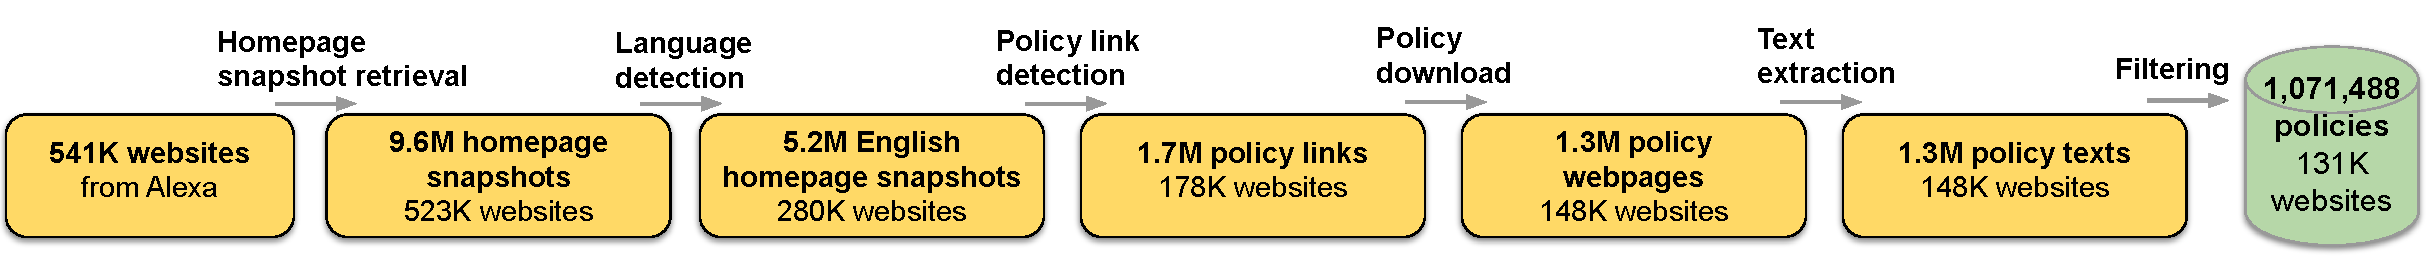
\includegraphics[width=0.99\textwidth]{chapters/privacypolicies/figures/data-collection-pipeline.pdf}
\caption{Overview of the data collection steps.}
%\Description[Data Collection Pipeline]{A flow diagram for our data collection pipeline. First we collect 541K websites from Alexa. Then we collect 9.6M homepage snapshots from 523K of those websites. We reduce this to 5.2M English homepage snapshots from 280K websites. We find 1.7M documents with privacy policy links from 178K websites. We find 1.3M privacy policy webpages from 148K websites. We extract text from 1.3M of those. Then we filter, leaving us with 1,071,488 policies from 131K websites.}
\label{fig:data-collection}
\end{figure*}

\subsection{Building the list of target websites}
\label{subsec:ppot:building-website-list}
We began by identifying a set of websites to include in our data collection process.
We chose websites that appeared in the Alexa top 100K list between 2009 and 2019. We considered 100K websites to be sufficient to reach into the long tail of the web, yet not so numerous as to pose computational challenges for data collection or analysis.

Next, we selected a method for discretizing time windows in our longitudinal dataset. We struck a trade-off between enabling granular analysis and limiting computational and storage requirements. For each website, we retrieved one snapshot from the first half of the year (January-June), and one from the second half (July-December). We call these six-month time spans~\emph{intervals}, and we use intervals as the basic time unit of our data collection and analysis. We refer to the first interval in a year as ``A'' and the second as ``B,'' so the first half of 2005 is ``2005A.''
For each interval, we used the daily archives of the Alexa top million list~\cite{naab2019prefix} to retrieve the Alexa rankings closest to the interval's midpoint: either March 31 (A) or September 30 (B).
We collected the Alexa ranks for each interval from the beginning of Alexa’s publication in 2009 to 2019.
We obtained 541,616 websites by combining all domains that appear in the top 100K of these 22 Alexa lists (two lists per year for 11 years).

\subsection{Building the list of snapshots}
\label{subsec:ppot:snapshot-retrieval}
Next, we determined the list of homepage snapshots available on the Wayback Machine
by querying their \emph{CDX Server API}~\cite{wayback-cdx-api}.
When a website had multiple snapshots in a six-month interval, we picked the snapshot closest to the midpoint of the interval.
We did not restrict our queries to a time window when searching for snapshots.
For instance, if {\tt example.com} was only listed in the Alexa top 100K in 2019,
we included its snapshots from any other year including as early as 1996, the first year for which Internet Archive has crawls~\cite{WaybackMachineGeneralInformation}.

\subsection{Downloading privacy policies}
\label{subsec:ppot:download-policies}
To download archived privacy policies, we built a custom crawler based on 
\emph{Pyppeteer}~\cite{miyakogi2019May}.


{\textbf{Language detection.}}
We limited ourselves to privacy policies in English, because our work is motivated by U.S. and EU developments and because evaluating privacy policies in other languages would require additional language proficiency. To exclude non-English websites from our crawls, we ran a language detection crawl that loaded the most recent homepage snapshot of each website, extracted the page text and identified the language of the extracted text using the \emph{Polyglot} Python library~\cite{polyglot-pypi}. If the latest snapshot failed to load, we tried to visit up to three random homepage snapshots to identify the site's language. 
We identified 280,798 English websites (5,223,228 snapshots),
and discarded the remaining 243,060 websites.


{\textbf{Loading the homepage snapshot.}}
To download archived privacy policies, we first loaded the homepage snapshot and ran a language check to make sure the snapshot was in English to account for changes in ownership or localization.
Second, we aborted visits where the crawler attempted to load the live (non-archived) version of the page or a snapshot from another interval due to a redirection.
Finally, we monitored all requests that the crawler made and blocked requests that attempted to fetch resources from live websites.

{\textbf{Privacy policy link detection.}}
Privacy policy links are not universally standardized in their text or URL.
We chose to use \textit{link texts}---that is, the clickable text appearing within the \texttt{<a>} element---to detect privacy policy links over other link features such as the URL path. Link texts are expected to be recognizable by users, and therefore more likely to contain certain keywords.

We detected policy links using exact and partial keyword matching.
We compiled these terms based on prior research~\cite{libert2018automated} and adding other terms by manually analyzing a sample of 100 pages where we did not find a privacy policy link in a pilot crawl. 
The manual analysis of these pages involved searching for privacy policy links and checking whether the linked page’s title, headers and content described a privacy policy or not. 

The link detection method is designed to be comprehensive and may lead to pages that do not contain actual privacy policies.
We detected and removed these false positives after the crawl (Section~\ref{sec:ppot:classifier}).

{\textbf{Policy download.}}
For each detected privacy policy link, we queried the Wayback Machine CDX API to retrieve the list of snapshots that were in the same time interval as the homepage snapshot. 
If the link URL ended in ``.pdf'', we used the Python \textit{requests} library~\cite{PyPI-requests} to retrieve the document.
If the link URL did not end in ``.pdf,'' we loaded the policy snapshot URL using the Pyppeteer-based crawler and ran a final language check to eliminate non-English policies.

{\textbf{Boilerplate removal and text extraction.}}
Privacy policy webpages typically include \emph{boilerplate} content that is separate from the policy (e.g., sidebars, footers, and headers). 
We removed boilerplate and extracted the main article from the page's DOM using the standalone version of Mozilla’s \emph{Readability} library~\cite{readability-mozilla}. 
Next, we extracted Markdown formatted text from the \emph{readable} policy web page using the \emph{html2text} Python library~\cite{html2text-github}. Markdown formatting allowed us to retain the links and basic document structure such as headers and lists, with minimal markup overhead.

\subsection{Practical and ethical considerations}
\label{subsec:ppot:practical-matters}
We confirmed that the Internet Archive’s terms of use do not prohibit automated access. Prior to starting our crawls, we sent an email to the IA’s contact address to notify them of our study.
We note that several prior works used Wayback Machine~\cite{lerner2016internet, lerner2017rewriting,brunelle2015not,brunelle2016impact}.

We took steps to minimize any adverse impact of our crawl on the Wayback Machine’s servers.
To reduce our bandwidth footprint, we disabled image downloads and limited the number of parallel crawl workers to 256.
We slowed down our crawls by pausing the workers when they received HTTP 429 (``Too Many Requests'') or HTTP 503 (``Service Unavailable'') errors from the Wayback Machine. 
After starting the crawl, we monitored the Wayback Machine server load stats~\cite{Wayback-Stats} to ensure that we were not imposing a significant load.

\subsection{Evaluating data quality}
\label{subsec:ppot:failure-analysis}

To ensure our dataset was of high quality, we manually investigated causes of failure (i.e., homepages where the crawler did not extract privacy policy text). We started with 5,223,228 homepage snapshots, and our crawler was able to download 1,292,420 privacy policy snapshots (24\%).
Downloads of privacy policies corresponding to the other 3,930,808 homepage snapshots failed due to various causes which we list in Table~\ref{tab:failure-cause}. While the high frequency of absent policies may be counter-intuitive, we found that only about 2\% of missing policies were attributable to crawler limitations.

The most common cause for a missing privacy policy, by far, was the crawler loading an archived homepage but failing to identify a privacy policy link.
The next most common cause was a~\emph{blank homepage}, where the crawler could not extract any text. Another recurring issue was that, though we had attempted to filter our non-English sites before the crawl, some homepage snapshots were classified as non-English.

To investigate the root causes of crawler failures, we manually analyzed 100 random snapshots for each of the most common crawl failures.
The main takeaways are:
only 4 of 100 homepages where the crawler did not identify a privacy policy link actually had a privacy policy link. Only 3 of 100 homepages detected as \emph{blank} contained a privacy policy link, while 13 contained some text in a separate frame--- typically old webpages. We further explore the relation between the snapshot age and crawl success in 
Section~\ref{subsec:ppot:data-overview}.

In sum, the overwhelming majority of crawl failures were attributable to homepage snapshots that did not contain a policy link, were not archived by the Wayback Machine (e.g., due to \texttt{robots.txt} rules), or were in a language other than English. The missing privacy policies that are attributable to limitations of the crawler are about 2\% of all snapshots (4\% of 44.7\% + 3\% of 7.3\%).


\begin{table}[t]
\centering
\resizebox{0.9\columnwidth}{!}{%
\begin{tabular}{@{}lrr@{}}
\toprule
\textbf{Failure cause}                           & \textbf{Count} & \textbf{Percent} \\ \midrule
No privacy policy link found on homepage         & 2,336,849      & 44.7\%       \\
Homepage detected as blank                        & 383,337       & 7.3\%      \\
Non-English homepage                             & 310,563        & 5.9\% \\
Policy page is not archived in this interval     & 271,736        & 5.2\%\\
Out-of-interval redirection for homepage         & 158,727        & 3.0\%\\
\bottomrule
\end{tabular}%
}
\caption{The five most common causes for the crawler to not download a privacy policy for a homepage. Out-of-interval redirection (row 5) means our crawler was redirected by the Wayback Machine to a snapshot in a different interval.}
\label{tab:failure-cause}
\end{table}


\section{Filtering the corpus}
\label{sec:ppot:classifier}

As discussed in Section \ref{subsec:ppot:download-policies}, we expect that some of the downloaded pages are not privacy policies. In order to filter out web pages that are not privacy policies, we trained a classifier on manually labeled data from the candidate policies. In this section, we refer to the text of the crawled web pages extracted with \emph{html2text} as \textit{documents}.

\textbf{Labeling definition.}
\label{subsec:ppot:pp-definition}
In order to label documents as privacy policies (or not), we needed to adopt a definition of what constitutes a privacy policy. We did not select a definition based on legal requirements, since both privacy policy text and applicable law can be ambiguous; we considered it outside the scope of the project to develop a classifier that accurately determines whether a document satisfies relevant legal requirements. Moreover, different jurisdictions have different legal requirements, which would necessitate further judgment about the applicable law for a given website.

Instead, we aimed to label whether a document is an \textit{apparent} privacy policy, without determining whether the document meets any particular legal requirements. Specifically, we labeled a document as a privacy policy if it met all of the following criteria:
\begin{itemize}
    \item The document relates to privacy. This criterion eliminates documents that are irrelevant, notwithstanding the link text.
    \item The document is legal in nature (e.g., uses legal terminology or appears to have legal significance). This eliminates documents that informally discuss privacy, such as blog posts.
\end{itemize}
In the course of applying our criteria, we encountered several recurring borderline types of documents. We labeled the following categories of documents as not privacy policies, because the contents were dissimilar or could otherwise be problematic for automated textual analysis.
\begin{itemize}
\item Incomplete privacy policies.

\item Cookie policies, which only describe the privacy practices of the website with respect to cookies.

\item Security policies, which only describe the security practices of the website.

\item Mixed documents containing paragraphs that are unrelated to privacy, such as a privacy policy intertwined with terms of service.

\item Privacy centers or landing pages, which further link to a privacy policy.

\item Privacy policy summaries, which further link to a long-form privacy policy.

\end{itemize}

\textbf{Labeling the sample.} We started by manually labeling a sample of candidate privacy policies (i.e., documents returned by the crawler) using our criteria. First, we randomly sampled and labeled 1,139 documents. In the sample, the majority of the documents 
matched the ``privacy + policy'' link text pattern (as described in Section \ref{subsec:ppot:download-policies}). We additionally sampled 50 random documents for each of the six remaining link text patterns so as to reduce overrepresentation of the 
dominant
link text pattern.

To confirm that the labeling was consistent with our criteria, two researchers independently labeled a sample of 100 randomly collected documents using the criteria above. The inter-annotator agreement was $\kappa=0.93$.

Our final labeled dataset contains 1,173 positives (i.e., documents that are privacy policies) and 266 negatives (i.e., documents that are not privacy policies), respectively $\sim$81.5\% and $\sim$18.5\%.

\textbf{Converting documents to features.} We cleaned the documents by removing Markdown tags and retaining inner text. We then removed symbols and the set of English stop words in \emph{scikit-learn}~\cite{scikit-learn}. Next, we created word n-gram tokens spanning from unigrams to 4-grams and generated features based on the frequency of occurrence of each token. We excluded tokens that appeared in fewer than 1\% of the documents.

We also extracted features from document titles, parsing them from the HTML \texttt{<title>} tag. For PDF files, we obtained titles by using the \textit{pdftitle} library~\cite{pdftitle-pypi}.
We removed symbols and stop words from the titles and we generated features based on the number of occurrences of each unigram in the title. We excluded tokens that appeared in fewer than 1\% of the documents.

We additionally extracted features from the link text and document URL. We found that these features did not contribute to classification performance, so we excluded them from our model.

\begin{figure}[]
\centering
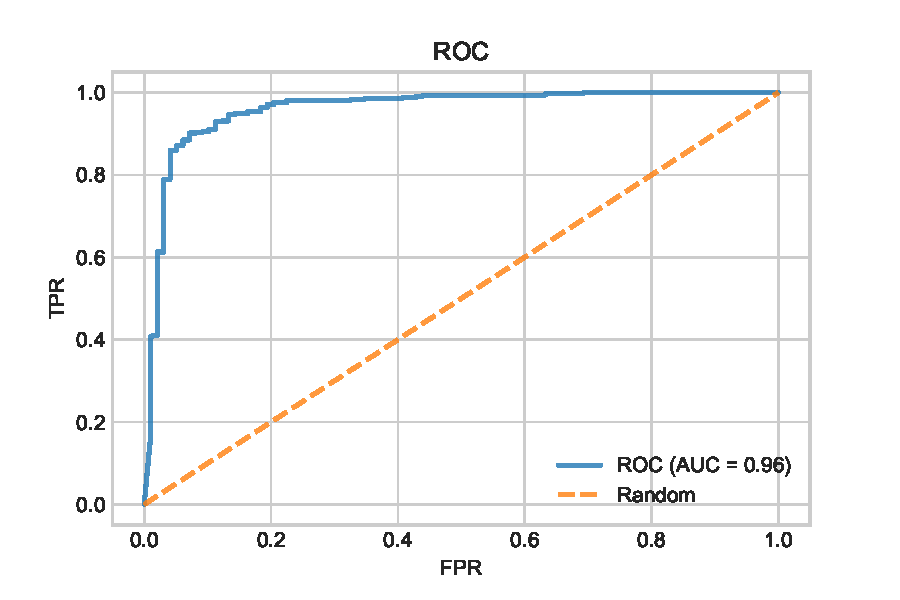
\includegraphics[width=0.8\columnwidth]{chapters/privacypolicies/figures/roc.pdf}
\caption[Predictive performance of the privacy policy random forest classifier]{Predictive performance of the privacy policy random forest classifier, applied to held-out documents.}
%\Description[ROC curve]{An ROC curve, with an AUC of 0.96}
\label{fig:roc-auc}
\end{figure}

\textbf{Model training and validation.}
We trained and tested two model types, random forest and logistic regression, using 10-fold cross validation across varying hyperparameters. We evaluated the models based on maximizing average area under the receiver operating characteristic curve (\textit{AUC}), since that metric accounts for the class imbalance. The best performing random forest model had a higher mean AUC than the best performing logistic regression model (97\% vs. 95\%), so we selected the random forest model.

We then considered the tradeoff between precision and recall for the random forest model. We manually selected a classification threshold that prioritized precision over recall, since we anticipate uses of our corpus (e.g., many forms of automated analysis) that may be more sensitive to erroneously including non-privacy policy documents than erroneously omitting privacy policies.

Finally, we evaluated our model on a held-out set of 749 randomly sampled and manually labeled documents, consisting of 651 positives and 98 negatives. The performance of the final model on the held-out set is shown in Figure \ref{fig:roc-auc}. The chosen classification threshold resulted in 97.9\% precision and 94.2\% recall.

\textbf{Document Classification.}
Approximately 17\% (220,932) of the documents in the dataset were classified as negatives, with the final dataset totaling 1,071,488 policies. We discuss the release of this data in Section \ref{sec:ppot:conclusion}.




\newcommand{\absentPerc}{80.0} %
\newcommand{\absentEngPerc}{61.3} %
\newcommand{\absentEngOneKPerc}{48.8} %
\newcommand{\gapsPerc}{81.8} %
\newcommand{\pregapsPerc}{76.5} %
\newcommand{\midgapsPerc}{7.4} %
\newcommand{\postgapsPerc}{16.1} %

\newcommand{\midgapsPossPerc}{29.8} %
\newcommand{\midgapsDomainsPerc}{54.1} %
\newcommand{\lifespanNoGaps}{11.2} %
\newcommand{\lifespanGaps}{16.5}

\newcommand{\numpresentdoms}{108,499} %
\newcommand{\numabsentenglishdoms}{150,192}



\newcommand{\midgapNoRankPerc}{3.0}
\newcommand{\pregapNoRankPerc}{78.4}
\newcommand{\postgapNoRankPerc}{11.2}
\newcommand{\allgapNoRankPerc}{92.7}
\newcommand{\notgapNoRankPerc}{7.3}

\newcommand{\percSnapshotWithPrior}{85.3} %
\newcommand{\percSnapshotWithoutPrior}{14.7} %


\newcommand{\corrMidgap}{-0.02} %
\newcommand{\corrPregap}{0.07} %
\newcommand{\corrPostgap}{0.08} %

\newcommand{\nSnapshots}{910,546}
\newcommand{\nSites}{108,499}


\section{Corpus composition}
\label{sec:ppot:dataset}

In order to understand the structure and biases of the data, we discuss the dataset composition.

\subsection{Cleaning the corpus}
\label{sec:ppot:deduplication}
In order to ensure the quality of our analysis, we purged additional, real policies from our dataset that might lead to a biased analysis. In total, we removed 160,941 policies following the steps listed below, leaving us with 910,546 policies from 108,499 sites. We call the resulting corpus the \textit{analysis subcorpus}. In sections \ref{sec:ppot:dataset}, \ref{sec:ppot:doclevstatstime}, and \ref{sec:ppot:analysis} we use the analysis subcorpus for our analyses.\footnote{While we removed this data for our analyses, we anticipate that there may be some research questions that would benefit from their inclusion. Accordingly, in our public release, we include both the full corpus and the analysis subcorpus.} 

\textbf{Parked domains.} As our dataset spans more than 20 years,
many domains have expired and were parked for monetization.
We found that privacy policies of the parking services such as {\tt godaddy.com} and {\tt hugedomains.com} were abundant in our dataset as they hosted privacy policies of 7,092 and 2,275 distinct domains, respectively.
We built a detection method based on the lists of domain parking services and registrars from prior research~\cite{vissers2015parking, kuhrer2014paint, kuhrer2014paint-TR, wang2006strider},
and the ICANN-Accredited Registrars list~\cite{ICANN-Registrars}.
With this method, we detected 79 parking providers and resellers and removed 24,289 (2.3\%) snapshots hosted by these providers.
 
\textbf{Homepage redirection.} In order to ensure the metadata is consistent with policy content, we removed policy snapshots with a cross-origin homepage redirection (COHR), unless both sites were likely owned by the same entity. Thus, we removed COHR policy snapshots, but we made an exception for websites with
common~\emph{label}s in their domain names (e.g. \texttt{google.com} and \texttt{google.ca})
as this may indicate that they are owned by the same organization.

\textbf{Policy URL.} Finally, to remove duplicates, we followed
Degeling et al.'s approach based on privacy policy URLs~\cite{degeling2018we}. When two or more sites shared a policy URL during the same interval, we kept only one, preferring the snapshot where the homepage domain matched the privacy policy domain. This removed 61,220 policies.





\subsection{Corpus overview}
\label{subsec:ppot:data-overview}

\begin{figure}[]
\centering
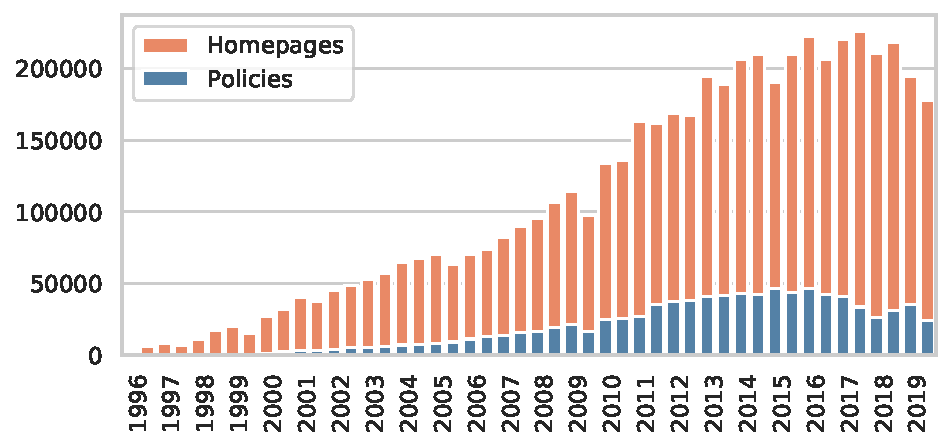
\includegraphics[width=0.99\columnwidth]{chapters/privacypolicies/figures/policy_homepage_counts.pdf}
\caption[The number of homepage snapshots and privacy policies for each interval]{The number of homepage snapshots and privacy policies for each interval. Note that each bar represents one interval and there are two intervals per year.}
%\Description[Bar plot of homepages versus policies, by year]{Generally, there are many more homepages than policies. The number of policies peaks in 2015 but declines slightly. The number of homepages roughly matches the same trend as the number of policies. }
\label{fig:numpolicies}
\end{figure}

On average, a website has 8.4 privacy policy snapshots ($M=6$). Although the dataset contains policies from as early as 1997, 79.4\% of the policies are from snapshots archived in 2010 or later.
As we briefly explored in Section~\ref{subsec:ppot:failure-analysis}, we expected the rate of successful downloads from earlier snapshots to be lower, in part due to different website structures, such as greater use of frames.

Figure~\ref{fig:numpolicies} shows the number of privacy policies and homepage snapshots per interval.
The decreases in the number of policies in 2009B and 2018A also occur in the number of homepage snapshots in those intervals, indicating that these decreases are due to changes in archiving or incomplete archives for those intervals.

\begin{figure}[t]
\centering
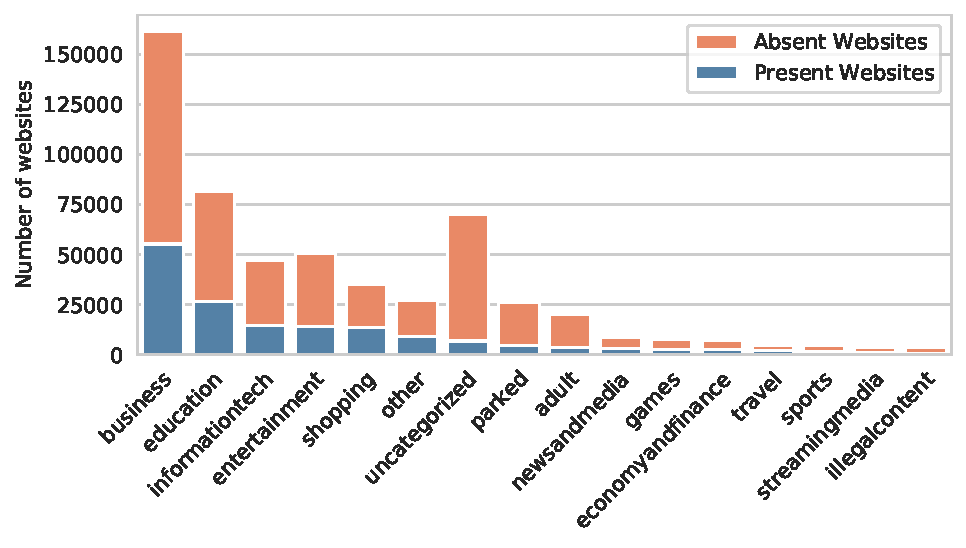
\includegraphics[width=1\columnwidth]{chapters/privacypolicies/figures/category_dist.pdf}

\caption[Distribution of website categories]{The distribution of website categories for present and missing sites. ``Other'' is composed of the 27 least frequent categories for English language websites. Websites which belong to multiple categories are counted once per category. Websites with no listed categories are added to the ``uncategorized'' category.}
%\Description[Histogram of category vs number of websites]{This diagram shows the number of websites that we tried to capture and that we succeeded in extracting an English language policy from. Categories in descending order: business, education, informationtech, entertainment, shopping, other, uncategorized, parked, adult, newsandmedia, games, economyandfinance, travel, sports, streamingmedia, illegalcontent.}
\label{fig:cat_dist}
\end{figure}

{\textbf{Distribution of website categories.}}
We examined the website categories for which we have the best coverage. We collected category data from Webshrinker~\cite{Webshrinker}, which provides a domain category lookup API.
Because category data is not available historically from Webshrinker, we assumed that categories are constant across time. We collected category data for the \numpresentdoms~websites in our dataset (present) and an additional \numabsentenglishdoms~websites with English homepages that were at one point in the Alexa top 100K (absent), which we show in Figure~\ref{fig:cat_dist}.
Just a few categories dominate both our dataset and English websites in general, and uncategorized websites are strongly underrepresented in our dataset.

{\textbf{Distribution of snapshot Alexa ranks.}}
The distribution of homepages and snapshots by Alexa rank is shown in Table~\ref{tab:rate-of-download-per-rank-bin}.
The $>1\text{M}$ bin contains snapshots for which we do not have an Alexa rank, either because they were not listed in the Alexa top 1M or were captured
before 2009.
While the majority of our policies come from websites with rank 100K and up, the success rate of obtaining a policy is much higher if the website is in the top 10K. 

\begin{table}[]
\centering
\resizebox{0.9\columnwidth}{!} \\ \midrule
(1, 1K{]}       & 13,455   & 5,003   & 37.2 \\
(1K, 10K{]}     & 104,801  & 38,959  & 37.2 \\
(10K, 100K{]}   & 980,928  & 278,324 & 28.4 \\
(100K, 1M{]}    & 1,339,157 & 319,866 & 23.9 \\
\textgreater 1M & 2,786,853 & 268,394 & 9.6  \\ \bottomrule
\end{tabular}%
}
\caption[Rate of successful privacy downloads by Alexa rank]{Rate of successful privacy downloads per Alexa rank buckets---based on privacy policies in the analysis subcorpus.}
\label{tab:rate-of-download-per-rank-bin}
\end{table}


\newcommand{\medianWCStartAlexa}{876}
\newcommand{\medianWCEnd}{1522}
\newcommand{\medianFKStart}{11.9}
\newcommand{\medianFKEnd}{13.2}

\section{Document-level trends}
\label{sec:ppot:doclevstatstime}

We examine how length, readability, and updates have changed over time. Because 
most of the privacy policies in our corpus are
from 2009-2019, we focus most of our analysis on that time range.

\subsection{Comprehension}
\begin{figure}[t]
\centering
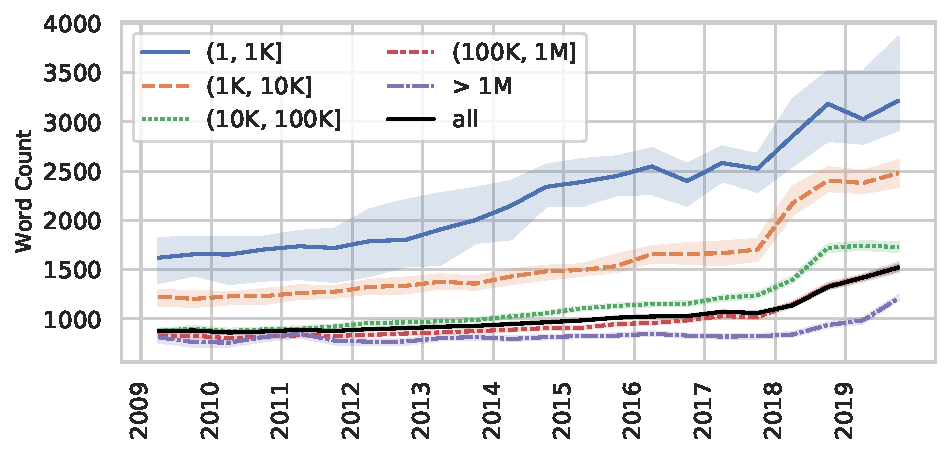
\includegraphics[width=0.99\columnwidth]{chapters/privacypolicies/figures/word-count-by-rank.pdf}
\caption{The median word count of policies binned by Alexa rank. The highlighted region in this and the following figures shows the 95\% confidence interval. Ranks are at the time of the snapshot.}
%\Description[Line plot of year vs word count]{The trend is generally slightly upwards and a similar shape across bins. Bins closer to 1 have more words.}
\label{fig:wordcount}
\end{figure}



{\bf Policy length.} Figure~\ref{fig:wordcount} shows the change in policy length as measured by word count. The median word count has increased gradually over time --- doubling between 2009A (\medianWCStartAlexa) and 2019B (\medianWCEnd) --- and more sharply in recent years, after the introduction of the GDPR. This trend holds for both popular and less popular websites. But the median hides a substantial variance: the 5\textsuperscript{th} percentile for word length is 248 words and the 95\textsuperscript{th} percentile is 3404 words. 
Our measurements for the top 10K are roughly consistent with the March 2016 measurements study by Degaling et al., but less so for their post-GDPR March 2018 measurements. Degaling et al. found the median privacy policy word count of the top 500 websites for 28 EU countries to be 2,145 in 2016 (our data: 1K: 2,691, 10K: 2,122) and 3,044 in 2018 (our data: 1K: 3,303, 10K: 2651) ~\cite{degeling2018we}. We believe the inconsistency is due to the difference in website sampling methods.




{\bf Readability.}
\label{sec:ppot:readability}
Several studies have shown that privacy policies are difficult to read~\cite{mcdonald2008cost,fabian2017large,milne2006longitudinal,li2012online}. 
Here we examine how readability has changed over time.
\begin{figure}
\centering
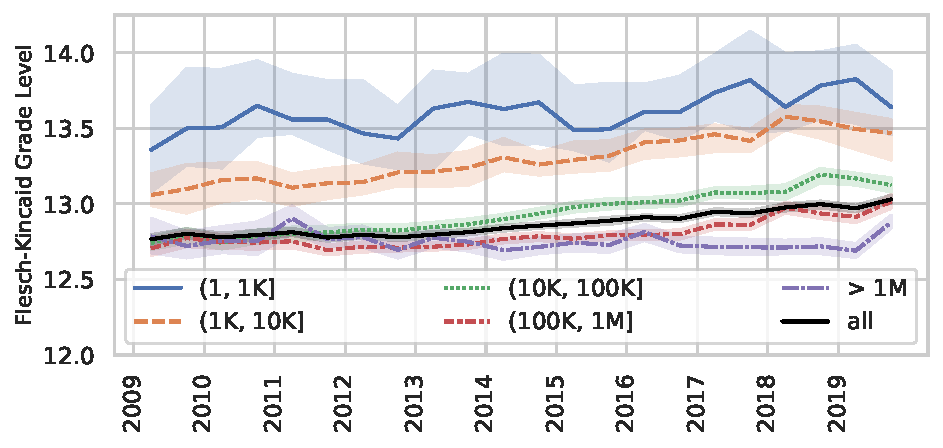
\includegraphics[width=1\columnwidth]{chapters/privacypolicies/figures/flesch_kincaid_dist.pdf}
\caption{Median Flesch-Kincaid grade level from 2009 to 2019, binned by Alexa rank. 
}
%\Description[Line plot of year vs Flesch Kincaid Grade level]{The trend is generally flat. Bins closer to 1 have a higher reading level.}
\label{fig:readability}
\end{figure}
We measured readability with the Flesch-Kincaid grade level (FKGL)~\cite{kincaid1975derivation}
using the \textit{py-readability-metrics} Python library~\cite{pyreadabilitymetrics}.
Our preprocessing involved removing non-sentence text such as headers, tables, and lists by writing a custom Markdown renderer using the \emph{Mistune}~\cite{mistune} Python library.

The FKGL measurements are shown in Figure~\ref{fig:readability}. The median readability score has risen more than a grade level from 2000A (\medianFKStart) to 2019B (\medianFKEnd). More popular websites have less readable policies.

In comparison, Li et al.~\cite{li2012online} measured the reading difficulty of privacy policies for websites for the 30 Dow Jones companies in 2012, finding an average FKGL of 13.33, which is similar to our findings for top 1K and top 10K websites.





\subsection{Privacy policy updates}
We measured the percentage of privacy policies updated in each interval.
To determine if these changes align with shifts in the language of privacy policies, we also measured terms that have experienced changes in their usage at each interval.

\textbf{Privacy policy updates.}
\label{sec:ppot:policy-updates}
\begin{figure}[]
\centering
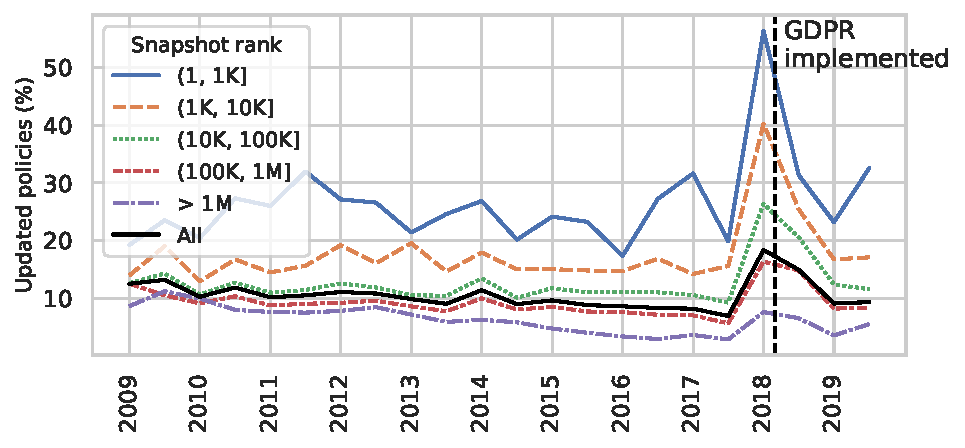
\includegraphics[width=0.99\columnwidth]{chapters/privacypolicies/figures/policy-updates.pdf}
\caption[Caption]{Percentage of privacy policies updated per interval.\protect\footnotemark}

%\Description[Line plot of year vs percentage of policies updated]{While jagged, the trends are relatively stable. Bins closer to 1 have more updated policies. There is a large spike shortly before GDPR is implemented.}

\label{fig:pct-policy-update}
\end{figure}
\footnotetext{We excluded snapshots for which we have a gap in the previous interval from Figure~\ref{fig:pct-policy-update}, since determining the exact time of the updates was not possible.}
Figure~\ref{fig:pct-policy-update} shows the percentage of updated policies, considering
only the~\emph{significant} updates, where the fuzzy similarity ratio~\cite{fuzzywuzzy} of consecutive policy snapshots is less than or equal to 95\%
~\cite{linden2020privacy}.
The spike in 2018 indicates the GDPR's substantial impact on privacy policies.  Although the figure shows that
popular websites update their policies more frequently,
the GDPR appears to have caused a major uptick across all rank buckets. 

\textbf{Change-point concentration.} 
To 
investigate the changes in privacy policy language and vocabulary,
we counted the number of n-gram frequency change-points detected by the PELT algorithm~\cite{killick2012optimal}, using the \textit{ruptures} library~\cite{ruptures}. Change point detection algorithms originate from the signal processing literature, and are designed to identify when a time-series signal has experienced a failure~\cite{picard1985testing}. In our case, n-gram frequency is the signal, and the ``failures'' are events that cause a shift in the usage.


We counted the number of change-points at each interval for lemmatized 1-grams and 8-grams with a document frequency of at least $0.01$ in at least one interval.
Figure~\ref{fig:changepoints} shows that the change points for n-grams concentrate around GDPR's introduction, following a similar trend to document level updates in Figure~\ref{fig:pct-policy-update}. This indicates that not only are websites updating their policies, but that the vocabulary used in privacy policies was forced to evolve due to the GDPR.


\textbf{Validation.} To verify that the increase in privacy policy updates we observed in 2018A was related to the GDPR, we took a list of GDPR-related phrases identified by Degeling et al.~\cite{degeling2018we}, plus the phrases “GDPR” and “General Data Protection Regulation,” and selected the subset of 20 phrases with a relative document frequency of less than 1\% in 2015A. We found that documents in 2018A containing at least one of these 20 GDPR-related phrases had a mean update length of 136 new lines, compared to 15 new lines in documents without these phrases, where “update length” is the number of added lines minus the number of deleted lines. The quartile boundaries were at, respectively, 0, 20, 129 and 0, 0, 0. This indicates that policies that contain GDPR-related terms were more likely to have a longer update in comparison to the prior version of the policy, supporting the link between the introduction of the GDPR and the increase in updates in 2018A.

\begin{figure}
    \centering
    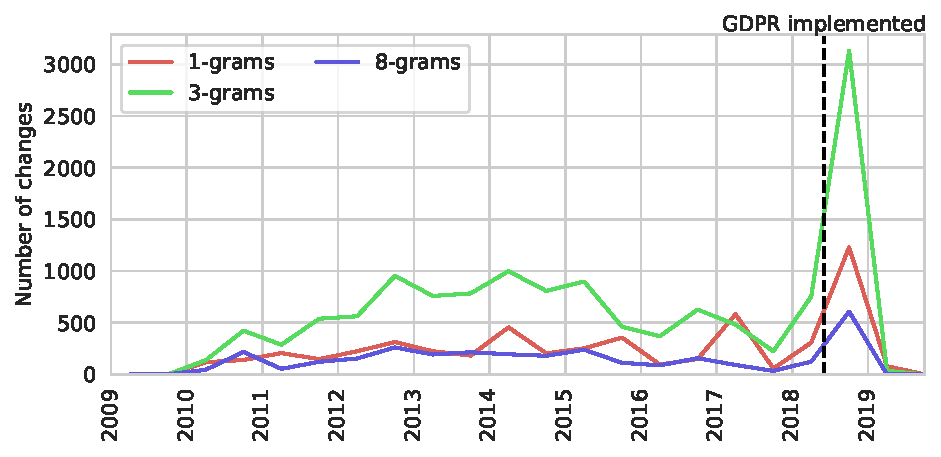
\includegraphics[width=.9\textwidth]{chapters/privacypolicies/figures/changepoints.pdf}
    \caption{Change point concentration. The y value is the number of frequent n-grams with change points in that interval for 1-grams, 3-grams, and 8-grams.}
    
%    \Description[Line plot of year vs number of changes]{There is a roughly arc shaped trend, with 3-grams being the most pronounced. There is a sharp spike right before GDPR is implemented.}
    \label{fig:changepoints}
\end{figure}

\section{Term-level trends}
\label{sec:ppot:analysis}

Motivated by our analysis of updates and change-points, we sought to understand how the language of privacy policies has shifted. While we followed prior research in our use of manually crafted keywords to analyze trends~\cite{degeling2018we},
we additionally developed a system to surface key terms that experts might otherwise overlook. Then we used the key terms surfaced by our tool to guide a more comprehensive analysis into specific concepts.

\subsection{Automated trend surfacing}
\label{sec:ppot:automated-trends}

We first built a pipeline to further clean and process the privacy policy texts. We started by replacing certain patterns---URLs, named entities using Spacy~\cite{spacy}, numbers, and emails---in the policies with placeholders. This allowed us to group together phrases that share the same template but include, for example, an organization name. We then extracted terms---n-grams, sentences, named entities, and URLs---for which we obtained the relative document frequency (the percentage of policies they appear in in an interval). Finally, we ranked terms of interest using a variety of scoring functions such as overall gain in relative frequency. 


\begin{table}[]
\centering
\resizebox{\columnwidth}{!}{
\begin{tabular}{rrr}
\toprule
\textbf{2-grams (Gain)}        & \textbf{Entities (Pos Slope 2)} & \textbf{2-grams (Pos Slope 2)} \\ \midrule
service providers (0.27) & gdpr (0.12)             & personal data (0.14)    \\
data protection (0.27)   & eu (0.11)               & data protection (0.13)       \\
personal data (0.24)     & google analytics (0.09) & withdraw consent (0.13)      \\
may include (0.24)       & eea (0.08)              & processing personal (0.13)          \\
may collect (0.22)       & facebook (0.07)         & legitimate interests  (0.12)     \\
\end{tabular}
}
\caption{The top five results from three categories of our automated trend surfacing tool. Scoring functions: ``gain,'' is the difference between the lowest and highest frequency; ``pos slope 2,'' is the maximum slope over any two intervals.}
\label{tbl:automated_results}
\end{table}
\begin{comment}
The trend surfacing tool is intended to surface terms of interest that experts can manually investigate.
It helps in two primary ways. First, it can help us ensure we have not missed any relevant terms during investigations.
Secondly, it can help identify candidate trends that we had not previously considered.
The results from the tool are actionable alone, but they can spark further investigation.\gnote{@RA: are we missing a NOT in the previous sentence?}
\end{comment}

\textbf{Results.} Our trend surfacing tool returned hundreds of phrases which we manually inspected. 
We provide some examples of top-scoring trends that our tool identified in Table \ref{tbl:automated_results}. Under 2-grams measured by gain, we note the growth of terms such as ``may include'' and ``may collect,'' which are terms of ambiguity in privacy policies (previously studied by Reidenberg et al.~\cite{reidenberg2016ambiguity}). This result suggests that privacy policies may be becoming more ambiguous over time, which should be investigated in future work. We noticed growth in terms related to European privacy regulation (GDPR, EU, EEA), along with Google Analytics and Facebook, two commonly used third-party services. We investigate this trend and other trends we observed in more depth in Section~\ref{subsec:ppot:trends}. Furthermore, we note growth in terms that likely relate to GDPR.


\subsection{Trends}
\label{subsec:ppot:trends}

After examining the results of our automated trend surfacing tool, we chose to investigate trends in three categories: self-regulatory bodies, tracking technologies, and third parties. We investigated tracking technologies because our tool identified several dozen terms of interest related to cookies and web beacons. Similarly, we included third parties as a category because our tool identified terms including Google, Facebook, Instagram, and Twitter. Furthermore, adequate disclosure in each of these categories is crucial to demonstrate the transparency that is a premise of \textit{notice and choice}. Finally, we chose to investigate self-regulatory initiatives because our tool identified several terms containing TrustArc, NAI, and DAA as gaining traction, which may be of interest to regulators.


\begin{figure}
    \centering
    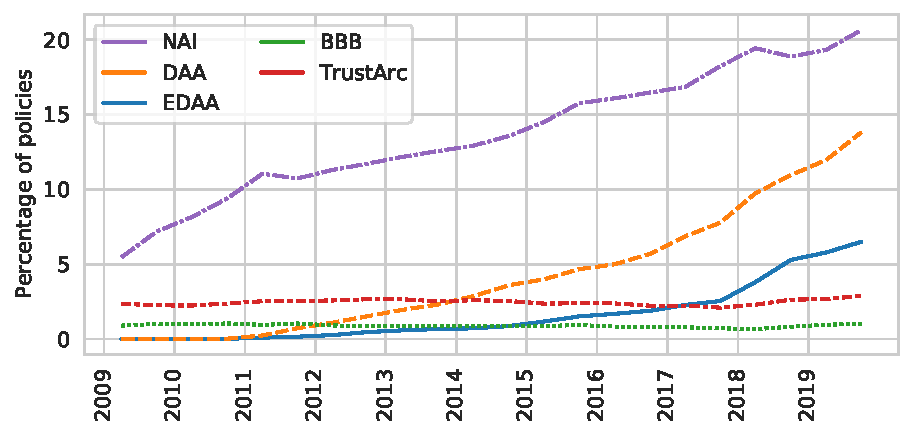
\includegraphics[width=0.9\textwidth]{chapters/privacypolicies/figures/selfreg.pdf}
    \caption[Self-regulation trends]{The percentage of policies, after deduplication, referencing self-regulation bodies over time. }
    
%    \Description[Line plot of year vs percentage of policies containing the trend]{The following terms trend roughly linearly upwards, in descending order of final value: NAI, DAA, EDAA. The following terms trend roughly flat: BBB, TrustArc.}
    \label{fig:selfreg}
\end{figure}


\textbf{Self-regulatory initiatives.} 
We began by identifying a set of self-regulatory initiatives. We chose six privacy seal vendors from prior work~\cite{rodrigues2013developing} and three advertising industry trade groups. We then measured how often privacy policies referred to these self-regulatory initiatives, counting a privacy policy as referencing an initiative if it either included the initiative's name or a link to the initiative's website.\footnote{We combined TrustArc and TRUSTe in our analysis, since they are the same entity. Our automated trend detection identified TrustArc as a term with increasing frequency, but when combined with TRUSTe the frequency of references is stable over time.} Figure~\ref{fig:selfreg} plots these references over time, omitting the initiatives that were mentioned in fewer than 1\% of privacy policies.

The graph indicates that self-regulatory online advertising trade groups---the Network Advertising Initiative (NAI), Digital Advertising Alliance (DAA), and European Interactive Digital Advertising Alliance (EDAA)---have seen substantial growth in mentions in privacy policies. The EDAA appears to have more than doubled its presence after the GDPR's introduction, and the NAI has risen around four-fold in 10 years.
By contrast, self-regulatory initiatives that are more commonly associated with first-party websites---
TrustArc and the Better Business Bureau (BBB)---have remained relatively stagnant over time.

\begin{figure}[t]
    \centering
    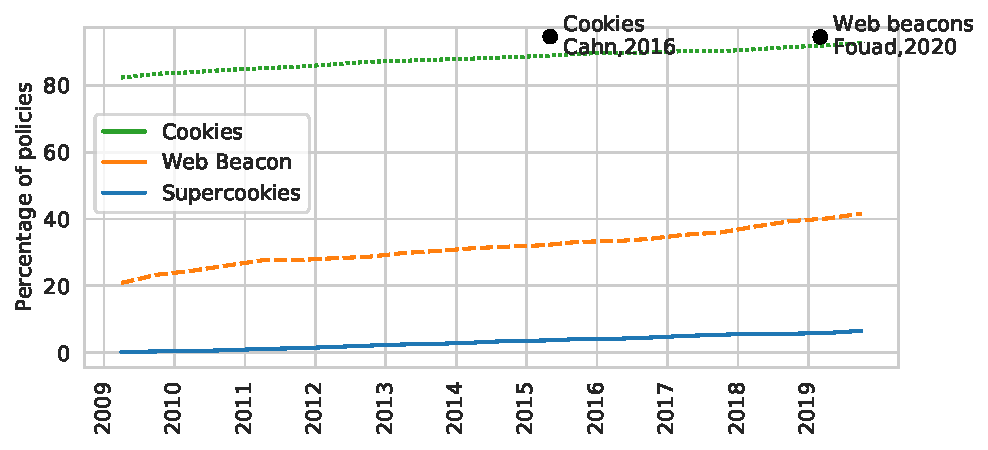
\includegraphics[width=0.9\textwidth]{chapters/privacypolicies/figures/technologies.pdf}
    \caption[Stateful tracking technologies trends]{The percentage of policies, after deduplication, that reference terms related to stateful tracking technologies. The dot labeled ``Cookies'' is the percentage of websites in the Alexa top 100K with any observed cookies~\cite{cahn2016empirical}. The dot ``Web beacons'' is the percentage of websites in the Alexa top 10K with observed pixels~\cite{Fouad2020missed}.}
%    \Description[Line plot of year vs percentage of policies containing the trend]{The following terms trend slightly upwards, in descending order of final value: cookies, Web Beacon, Supercookies. Other researchers measurements for cookies approximately match the value at that point.}
    \label{fig:trackingtech}
\end{figure}

\begin{figure}[t]
    \centering
    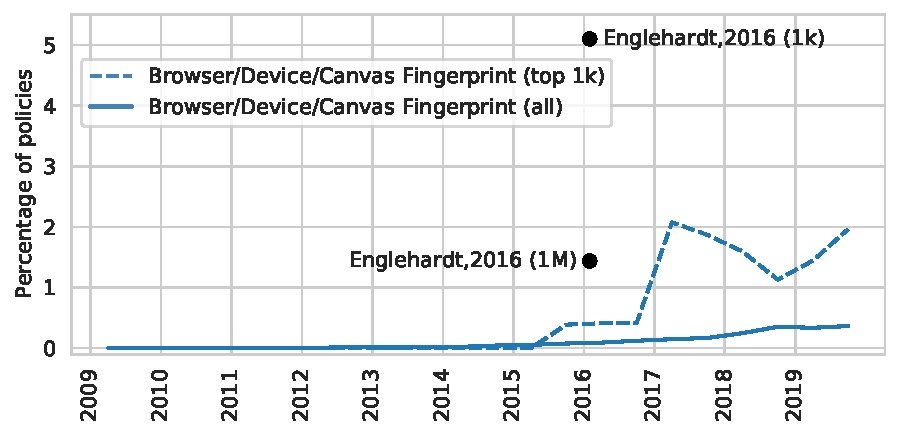
\includegraphics[width=0.9\textwidth]{chapters/privacypolicies/figures/fingerprinting.pdf}
    \caption[Fingerprinting trends]{The percentage of policies, after deduplication, that reference terms related to fingerprinting. The dot labeled ``1K'' is the percentage of websites in the Alexa top 1K at the time with observed canvas fingerprinting, and ``1M'' is the top 1M~\cite{englehardt2016online}.}
%    \Description[Line plot of year vs percentage of policies containing the trend]{This graph shows Browser/Device/Canvas fingerprinting for all against the top 1k. The top 1k grows faster than all, peaking, then dropping, one year after Englehardt et al., 2016.}
    \label{fig:fingerprinting}
\end{figure}

\textbf{Tracking technologies.} Tracking technologies are pervasive in the modern web~\cite{englehardt2016online}. If privacy policies were fully transparent, we would expect that observations of tracking technologies on the web would match mentions in privacy policies, so we investigated how frequently privacy policies disclose the use of tracking technologies. 

Using our automated trend surfacing tool as a guide, we selected four terms related to tracking technologies, which we split into two categories: stateful tracking technologies and stateless (``fingerprinting'') tracking technologies~\cite{mayer2012}. We constructed regular expressions to match all names listed in the respective Wikipedia entry for the technology~\cite{wikipediaCookie,wikipediaWebBeacon,wikipediaDeviceFingerprint,wikipediaCanvasFingerprint,wikipediaLSO,wikipediaEvercookie}.
The percentage of privacy policies containing the first and second
groups are shown in Figure \ref{fig:trackingtech} and Figure~\ref{fig:fingerprinting}, respectively. Mentions of ``cookie'' are quite close to the observations of the usage of cookies by Englehardt and Narayanan~\cite{englehardt2016online}, and Cahn et al.~\cite{cahn2016empirical}. However, web beacons and fingerprinting appear to be underreported. Fouad et al. measured that 94.6\% of the Alexa top 10K websites had web beacons~\cite{Fouad2020missed}, compared to 25.8\% of policies in 2019 mentioning the related terms. Further, fingerprinting related terms were mentioned far less commonly than Englehardt and Narayanan's measurements of canvas fingerprinting in both the top 1K and top 1M~\cite{englehardt2016online}.

\begin{figure}
    \centering
    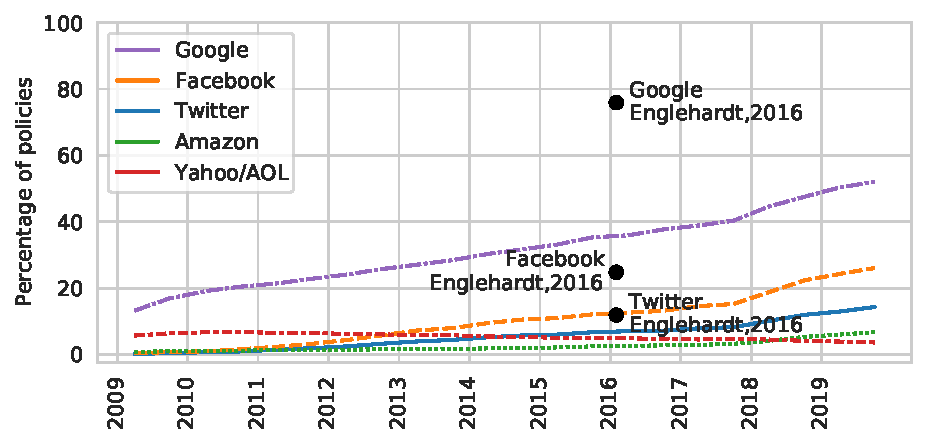
\includegraphics[width=0.9\textwidth]{chapters/privacypolicies/figures/trackers.pdf}
    \caption[Third party trends]{The percentage of policies, after deduplication, that reference specific third parties. A match for a common name for the third-party organization, or a match in a link for any domain owned by the third-party organization or their parent organization was considered a reference. Dots indicate measurements of the presence of third parties as a tracker~\cite{englehardt2016online}.}
%    \Description[Line plot of year vs percentage of policies containing the trend]{The following terms trend upwards, in descending order of final value: Google, Facebook, Twitter. The following trends remain flat: Amazon, Yahoo/AOL. Measurements for Twitter from Englehardt et al. are larger but somewhat close to policy mentions. Measurements for Facebook and Google are substantially larger.}
    \label{fig:trackers}
\end{figure}

\textbf{Third parties.} Third-party services are often associated with tracking users on the web~\cite{englehardt2016online}. Continuing our investigation of disclosure and transparency, we chose to examine how often privacy policies disclose the prevalence of third parties.

We compiled a list of 20 popular third parties from other measurements of third parties on the web~\cite{trackerradar, englehardt2016online,lerner2016internet}. We searched for alternative names for each third party and domain names operated by the third party using data from DuckDuckGo's Tracker Radar project~\cite{trackerradar}. We chose the top five most referenced third parties in 2019B, which we show in Figure~\ref{fig:trackers}. We found that these third parties were mentioned in privacy policies far less frequently than they were observed in the web measurements~\cite{trackerradar,englehardt2016online}. 

The gap between observation and disclosure indicates that many privacy policies may not be disclosing all present third parties. 
We note that reporting of third parties is largely increasing. It is unclear if this is due to increased presence or transparency.

\textbf{Validation.} We evaluated our matching criteria for tracking technologies, third parties, and self-regulatory initiatives, to ensure that we were studying the intended trends. Table \ref{tab:selfreg-NDE-labeled} presents results from manually labeling 100 positive examples of each matching category, showing that our matching criteria have high precision.

{
\begin{table}[]
\centering
\resizebox{0.8\columnwidth}{!}{%
\begin{tabular}{@{}lcc@{}}
\toprule
\textbf{Query} & \textbf{Positive} & \textbf{Negative} \\ \midrule
Cookies & 99 & 1\\
Web Beacon & 89 & 11\\
Supercookies & 99 & 1\\
Browser/device/canvas fingerprint& 100 & 0\\
\midrule
Google & 95 & 5\\
Facebook & 86 & 14\\
Twitter & 73 & 27\\
Amazon & 86 & 14\\
Yahoo/AOL & 97 & 3\\
\midrule
TrustArc & 87 & 13\\
BBB & 97 & 3\\
NAI & 95 & 5\\
DAA & 100 & 0 \\
EDAA & 100 & 0\\
\bottomrule
\end{tabular}%
}
\caption{Manual validation of 100 positives for each query. For third parties and tracking technologies, positives indicate the term is used in a context related to tracking. For self-regulatory initiatives, positives indicate a relationship with the initiative.}
\label{tab:selfreg-NDE-labeled}
\end{table}
}

\begin{table}[]
\centering

\resizebox{\columnwidth}{!}{
\begin{tabular}{@{}lrl@{}}
\toprule
\textbf{Privacy policy URL} & \textbf{\# of websites with linking policy} &  \\ \midrule
google.com/privacy\_ads.html & 11,324 &  \\
google.com/intl/en/policies/privacy & 1,690 &  \\
google.com/policies/privacy & 1,421 &  \\
automattic.com/privacy & 948 &  \\
twitter.com/privacy & 931 &  \\
google.com/privacy.html & 873 &  \\
facebook.com/policy.php & 607 &  \\
google.com/privacypolicy.html & 559 &  \\
mailchimp.com/legal/privacy & 528 &  \\
doubleclick.net/us/corporate/privacy & 498 &  \\ \bottomrule
\end{tabular}
}
\caption{Privacy policies that are most linked from the other privacy policies. The right column indicates the distinct number of sites.
}

\label{tab:most-linked-policies}
\end{table}
\textbf{Outbound links.} In addition to disclosing third-party partners, companies may provide links to opt-out pages, industry organizations, or third-party partners that they share data with. Analyzing links found in the privacy policies may reveal trends in third-party data sharing and the effect of regulation on transparency. Here we study links from one privacy policy to another.

We found that 20.3\% of websites link to one or more additional privacy policies. 
This result implies that users wishing to achieve a comprehensive understanding of a website's data practices face an increased burden of reading both the first-party policy and the linked policies.
We show the ten privacy policy URLs with the most incoming links from other policies in Table \ref{tab:most-linked-policies}, which includes six policy URLs from Google. 
  
The privacy links we observe provide an alternate explanation to the disparity we observed in our discussion of tracking technologies
---specific technologies may not be named because they are explained in the third party's privacy policy---instead of the first party's. 




\section{Conclusion}
\label{sec:conclusion}
We developed a system for the longitudinal, large-scale, automated collection and curation of privacy policies. Using the system we built a dataset of over 1M privacy policies that span more than two decades. We found that privacy policies are becoming longer and harder to read.

We developed an automated trend surfacing tool and investigated some of the surfaced trends. Specifically, we investigated trends around third parties, tracking technologies, and self-regulatory bodies. Our results suggest that privacy policies show a concerning lack of transparency: the usage of third parties and tracking technologies is severely underreported.

Our results add to the growing body of evidence suggesting the inadequacy of the ``notice and choice'' model for privacy policy regulation and demonstrate the monumental impact of the GDPR.


\textbf{Release.} Our dataset and source code is available for public use.\footnote{ \url{https://privacypolicies.cs.princeton.edu/}} The access requests we have received have revealed a diversity of use cases for our data, including the study of responses to regulation, automated enforcement, health information technology, and ethics.

In addition to making data and code available, inspired by the TOSBack project~\cite{TOSBack}, we built a chronologically accurate GitHub repository of the policy documents in our dataset.
We used \emph{GitPython}~\cite{GitPython} to commit privacy policy texts and HTML sources (in a separate branch) using the time-of-archive timestamps and detailed privacy policy metadata. 
GitHub’s easy to use web interface enables users without technical skills to perform full text search, compare different versions of the same policy, or use the ``Blame’’ feature to trace modifications.
Finally, we built a separate web interface
to make it easier to search, filter, and explore the privacy policies in the GitHub repository.


\textbf{Limitations.}
Our data collection and analyses were limited to privacy policies; we did not analyze how archived websites track users or share personal data with third parties. 

For internationalized websites, the location of the Wayback Machine crawlers could determine the language of the archived site and its privacy policy. 
Although ``the vast majority of captures are initiated from the [United States],'' there is no way to determine the location, country, or IP address of the Wayback Machine crawlers that captured a particular snapshot~\cite{crawl-location-tweet-by-graham}.


For our readability discussion, we noted that readability metrics have limitations; they do not consider organization, formatting, or length of the document, nor the semantic difficulty of the document. 

In our discussion of how terms trend over time, we used (typically handcrafted) regular expressions to search for referenced terms. Despite our best efforts and extensive manual validation, these regular expressions may capture terms that we did not intend to capture. They additionally may capture terms we intended to capture, but do not fit the targeted concept, and they may miss terms that fit the targeted concept. 


\textbf{Future work.}
Based on our results we suggest several directions for future work. The reporting gap for third parties and tracking technologies could be investigated with a combination of web measurements and privacy policy analysis. Another direction is to further investigate ambiguity in privacy policies.

More sophisticated natural language processing techniques applied to longitudinal privacy policy data could improve our understanding of how online services adapt to new privacy regulations, the prevalence of specific business practices, and whether online services are complying with privacy laws. 
We anticipate that our dataset will prove useful for research in all of these directions.

\chapter{Reviews in motion: a large scale, longitudinal study of review recommendations on Yelp}


%Mukherjee dataset
\newcommand{\MukherjeeRestaurantCt}{130}
\newcommand{\MukherjeeHotelCt}{85}
\newcommand{\OurRestaurantCt}{129}
\newcommand{\OurHotelCt}{79}
\newcommand{\MukherjeeReviewMatchPerc}{91.8\%}

%Reclassification data
\newcommand{\RecToFil}{3.9\%}
\newcommand{\FilToRec}{41.3\%}

%Filtered amounts
\newcommand{\OriginalFilteredPercentage}{12.5\%}
\newcommand{\NewFilteredPercentage}{11.6\%}


\section{Introduction} \label{sec:rim:introduction}

%\raNote{discussion order should be longitudinal $\to$ reclassification}

%\raNote{six year gap $\to$ eight year gap!}

%\raNote{The abstract is more detailed than the intro -- fix that (second paragraph of contributions)}

Online reviews are an important source of consumer information, and they have a substantial impact on businesses' economic outcomes~\cite{luca2016reviews,anderson2012impact}. This creates incentives for various parties to engage in problematic reviewing practices~\cite{streitfeld2012buy,miller19plastic}. These problematic reviews can encompass a large spectrum of behaviors, such as the creation of new accounts for posting fake reviews, hijacking legitimate accounts, compensating real users for posting favorable reviews, incentivized reviews, reviews written by friends or competitors, or reviews that are not relevant to the product or service, and they are the subject of ongoing interest to regulators~\cite{jindal2008opinion,yelpwhyrec,ftc21notice}. To address the challenges posed by such problematic reviews, review platforms have created classification systems to present users with the best reviews to make informed decisions. A wealth of prior work has taken a variety of approaches to understanding online reviews and the underlying classification systems. This work ranges from studying the factors motivating both honest and problematic reviews to how to detect and generate opinion spam or fake reviews~\cite{jindal2008opinion,yoo2008motivates,baginski2014exploring}. Most of this work examines reviews and review classification systems from a single time-point; however, this perspective is an incomplete one---these classification decisions are not static.

%The overwhelming majority of prior work has focused on analysis of reviews from a single snapshot in time. Using this approach, prior work has tried to detect fake reviews, explored demographic effects on reviews, studied the incentive structures behind reviews, and more. Some prior work has focused on identifying parameters that predict an existing platform's problematic review classifier, allowing some reverse engineering of existing classifier~\cite{mukherjee2013yelp}, but the question remains as to how accurate, effective, and stable this classifier is. We believe this is a crucial gap in the literature, and that more deeply understanding the existing review filters can help us understand their impact, the challenges faced in design and implementation, and help all platforms improve their classifiers.

\textbf{Contributions.} In this work, we move from a view of reviews at rest to a view of reviews in motion: how do reviews move between classes? We explore the dynamic classification of reviews through the collection and analysis of three novel, longitudinal datasets, focused on Yelp. We sought to observe the changing nature of review classification, and thus we collected datasets in which we observed the reviews for a fixed set of businesses across multiple time-points. Our datasets total over 12.5 million total and two million unique reviews, with observations over timescales ranging from four months to eight years. The longitudinal aspect of data allows us to observe the movement of reviews between classifications, which we call ``reclassification''. We take advantage of our dataset to study other aspects of online reviews: our carefully chosen cross sections allow us to approach questions of demographic interactions with reviews, and our timing allows us to explore questions around COVID-19's impact on reviews.

Our results demonstrate that reviews are routinely reclassified, in between both the ``Recommended'' and ``Not Recommended'' classes, occasionally multiple times. Understanding these reclassifications helps to highlight the uncertainty in Yelp's classifier---whether that's because of insufficient information or imperfect models---and the challenging nature of building robust classifiers. They also act as a potential point of frustration or even chilling for legitimate users and businesses.

Our contributions are as follows:
\begin{enumerate}
    \item The largest longitudinal dataset of reviews, tracing over 2M reviews across over 11k businesses.
    \item The first study of review reclassification and exploration of the phenomena. We find reclassification rates between 0.54\% over four months to 8.69\% over 8 years. Furthermore,  newer reviews are more affected, and that classification appears to happen mostly at an author-level.
    \item An exploration into the impacts of income and density, showing disparities in review frequency and reclassification by both income and density.
    \item An investigation  the impacts of mask discussion and rules, showing that the classifier largely erases rating differences for businesses requiring masks.
\end{enumerate}% \raNote{make sure to fact check these claims}



\section{Related work} \label{sec:related_work}

Extensive academic literature from multiple disciplines studies online reviews and fake reviews. We highlight four primary areas of prior work: longitudinal study of reviews, demographics and reviews, problematic reviews, and incentives for reviewing.

\textit{Longitudinal study.} Some researchers have performed longitudinal analyses on reviews with a single snapshot, for example by using review dates~\cite{bakhshi2014demographics,ye2016temporal,wang2017temporal}.  Other studies have linked datasets together to gain a better vantage on the review landscape, but still rely on a single snapshot for each data point. For example, \citet{nilizadeh2019think} used reviews from multiple different review platforms along with change point analysis to find fraudlent reviews. To the best of our knowledge, no other studies focus on review reclassification. Yelp acknowledges that reviews are classified by an automated system and sometimes reclassified, but Yelp does not disclose the frequency with which this happens \cite{yelpwhyrec,yelpwhychange}.

\textit{Demographics and reviews.} Ensuring equal access to and treatment by technology is an important equity issue. Two areas of concern are the rural/urban divide and income inequality. \citet{baginski2014exploring} explored the hypothesis that, within Franklin County, OH, low income areas have fewer reviews. Instead, they found that there were strong concentrations of reviews, and suggested that technological adoption may play a role. Van Velthoven et al.~\cite{van2018cross} support this hypothesis in their work exploring reviews and ratings in a medical setting; they also do not find a strong link between income or urban/suburban living and the frequency of review authorship. In contrast, \citet{bakhshi2014demographics} find that, among restaurant reviews, local population density has a small but statistically significant effect on review count, but not on rating.  However, \citet{sutherland2020topic} show, using topic modelling, that in hotel ratings rural and metropolitan settings and decor are important discussion points for consumers. Our work helps improve the perspective on how demographics shape reviews.

\textit{Problematic reviews.} Problematic reviews have served as a persistent challenge in the review landscape, largely in the context of detecting fake reviews. \citet{ott2012estimating} estimated that fake reviews occurred at a rate of 2-6\% across six platforms, but other estimates of fake reviews reach 50\%-70\%~\cite{dwoskin2018merchants,elliott2018trust}. Yelp reports filtering about one quarter of its reviews~\cite{yelp2010recommend}. A wealth of research focuses on the problem of detecting these fake reviews~\cite{jindal2008opinion,martens2019towards,ye2016temporal,shehnepoor2017netspam,kumar2018rev2,harris2012detecting,mukherjee2013yelp}. Some works have taken an adversarial approach, generating fake reviews rather than detecting~\cite{adelani2020generating,juuti2018stay,yao2017automated}.

One challenge in analyzing fake reviews is the absence of ground-truth data. Fake reviews may be designed to fool even humans~\cite{ott2011finding}, and only the author of a review may know its authenticity with certainty. \citet{wang2016real} obtained ground-truth data by using leaked data from fake reviewers. \citet{martens2019towards} posed as customers to fake review providers to identify other fake reviews. \citet{ott2011finding} had study participants create fake reviews. Other studies rely on suspected---but unconfirmed---fake reviews. ~\citet{jindal2008opinion} used ``obviously'' fake reviews (e.g., duplicates) on Amazon to train a model to find other fake reviews. \citet{mukherjee2013yelp} and \citet{rayana2015collective} rely on Yelp's classifications for analysis.% By studying how output of the classifier, we sidestep the need to know definitively whether individual reviews are fake or otherwise problematic.

In contrast to most of these works, our work studies Yelp's deployed classifier which is designed to filter out such reviews, particularly focusing on the dynamic nature of decisions made.% \raNote{polish language}

\textit{Incentives.} A number of economics studies have tried to understand the incentives behind both posting reviews and restaurants reviews. \citet{yoo2008motivates} showed that most consumers post reviews for themselves, to help the company, and to protect other consumers, while a smaller portion do so as retribution for poor service. \citet{luca2016fake} studied the economic incentives for problematic review posts, concluding that chain restaurants, restaurants with stable ratings, and restaurants with not much competition are less likely to post fake reviews. This literature is crucial for interpretation of the results of our study.

%\raNote{Mention longitudinal}

%\cite{baginski2014exploring} -- study of franklin county, oh reviews, rejected hypothesis that low income areas have fewer reviews, but they still find that reviews are concentrated in specific areas



%\cite{sutherland2020topic} -- rural/urban settings are important features in hotel review discussions, therefore likely have an impact on business success and choices

%\cite{van2018cross} -- studied a number of factors wrt medical review reading and writing. found that income and urban/suburban are not strongly correlated with medical review authorship; internet use was the only factor they found

%\cite{nilizadeh2019think} -- linked reviews from different sites and used change point analysis to find fraudulent reviews

%\cite{luca2016fake} -- studieid the economic incentives of reviews on yelp. certain types of restauraunts, specifically chains, are less likely to commit review fraud. more competition leads to increases in RF
\section{Data collection} \label{sec:dataset}

We collected and constructed three longitudinal datasets to study reviews on Yelp. We present background on Yelp in Section \ref{subsec:background}, we describe the difference between our three datasets in Section \ref{subsec:target_set}, and we describe our crawling process in Section \ref{subsec:crawling}.




 
% \raNote{If Roland gets an arXiv paper up before the deadline, maybe we can cite that here}

\subsection{Background} \label{subsec:background}

Yelp breaks reviews into two primary categories, assigned by a software classifer. The categories are ``Recommended'' and ``Not Recommended''. Yelp lists four reasons for classifying a review as ``Not Recommended'': conflicts of interest, solicited reviews, reliability, and usefulness. Not Recommended reviews do not affect metrics and are displayed less prominently than Recommended reviews~\cite{yelpwhyrec,yelprecommendationsoftware,yelpstarrating}. In order to study the classifier, it is important that we collect both Recommended and Not Recommended reviews. Yelp also shows a third class: ``Removed for Violating our Terms of Service'', which we do not use in our analysis. While Yelp has published an official review dataset for academic purposes~\cite{yelpacademicdataset}, this dataset is not up-to-date and does not include Not Recommended reviews.

We chose to study Yelp because prior work had established reference datasets we could compare against; we chose to use \citet{mukherjee2013yelp}'s dataset of Yelp reviews, collected in 2012, which contains both Recommended and Not Recommended reviews from around 200 restaurants and hotels in Chicago.
%\pmNote{why did we choose this? what is this dataset about}
Furthermore, unlike many other platforms, Yelp allows access to reviews that it does not recommend.

%\pmNote{Shouldn't this para preceed the discussion of Mukharje et al?}






\subsection{Target set selection} \label{subsec:target_set}
Selecting the target set, the set of zipcodes or businesses to study, required careful selection of sample.


\textbf{Coarse crawl (EYG).} 
The first dataset was a single crawl in which we recrawled the same businesses focused on by \citet{mukherjee2013yelp} Thus, our sample was fixed by the original crawl. Specifically, the Mukherjee et al. crawl collected all businesses from a target set, then collected all reviews from the authors posting reviews on the targeted businesses, finally they collected metadata for the businesses from those posts. We re-crawled Mukerjee et al.'s target set of businesses, since those are the businesses for which the we have the most complete data. We call this the ``eight year gap (EYG)'' crawl because Mukherjee et al. performed their crawl in 2012 and we performed ours in 2020. By comparing our crawl against Mukherjee's crawl, we are able to observe reclassifications in the reviews.

%\pmNote{somewhere in this discussion, we need to make it clear that the metadata information we are collecting about the reviews includes recommended or not recommended status. also, we need to make it clear that comparison between Mukharjee's dataset and our dataset allows analysis of the dynamics of Yelp's classifier, by observing change in classification outcomes for reviews} \raNote{I added a table in Appendix A that I think should address the collected information. It's referenced in Section \ref{subsec:crawling}}

\textbf{Fine crawl (CHI).}
%\pmNote{why do we need a second crawl? what problem are we trying to solve?}
While our coarse dataset shows changes over a long time scale, it does not reveal how frequently reclassifications occur. To address this, we built a second, finer grained dataset by repeatedly collecting reviews 8 times over 11 months. We chose to use the same zipcodes so that there would be some intersection with the EYG crawl businesses, helping contextualize those businesses, ensuring continued crawling of some EYG crawl businesses. Because the zipcodes are within a single metropolitan area, the Chicago area, we call this the ``Chicago (CHI)'' crawl. This more comprehensive but localized coverage of reviews allows for authors to be observed posting multiple reviews.

\textbf{Population Density and Income (UDIS / UDS \& UIS).}
Our fine grained dataset gives insight into a local review ecosystem, but it is possible that the sample chosen is not a representative sample. To address this, we collected a third dataset to obtain a broader range of reviews across the US. To allow for study of the impact of reviews in a diverse set of regions, we stratified regions along two axes: one of density, one of income. 
%\pmNote{when we say density, should we instead say population density?}
We collected density and income information from the US census~\cite{acs2019householdincome}, and used ZipCode Tabulated Areas (ZCTAs) as a proxy for zipcode. ZCTAs approximate USPS ZipCodes, and typically, but not universally, match them~\cite{census2020zctas}.

For the density stratified crawl, we stratified zipcodes into 5 strata, dividing the strata evenly by population, using US census data for population estimates~\cite{acs2019populationtotal}. We uniformly sampled zipcodes from each strata until we had sampled at least 500 businesses from that strata, using the Yelp Fusion API to help us determine how many businesses were in each zipcode. We then collected 4 monthly crawls of each dataset. We repeated the same process for the income stratified crawl.

The strata for the income crawls are: \$0--\$55k, \$55k--\$68k, \$68k--\$82k, \$82k--\$105k, \$105k--\$250k. The strata for the density crawls are: 0--67 ppl/$\text{km}^2$, 67--302 ppl$/\text{km}^2$, 302--881 ppl$/\text{km}^2$, 881--1,873 ppl$/\text{km}^2$, 1,873--57,541 ppl$/\text{km}^2$.

Since the union of the income and density data is also a useful dataset as broader sample than the CHI dataset, we present some analyses with individual datasets, ``US Density Stratified (UDS)'' and ``US Income Statified (UIS)'', and some with the combined dataset, ``US Density and Income Stratified (UDIS)''.

\subsection{Crawling}\label{subsec:crawling}


% \pmNote{awkward to begin a subsection with a forward reference to the appendix. lets push this a bit later in the text}
% \raNote{Might be good to discuss this tomorrow if you have time -- currently don't have space for the figures in the text}
% \pmNote{regardless, the forward reference can be moved to the end of the para}
Our crawling occurs in two phases.
First, we have an initial setup phase to collect the set of businesses to crawl. 
%\pmNote{the sentence is very vague. what does the setup phase do?}
Then when have a crawl phase, where we repeatedly collect reviews. At each crawl timepoint, we visit each each of the targeted businesses to collect all reviews on that business. We provide an overview of our crawling process in Appendix \ref{apd:collection}, Figure \ref{fig:crawling_diagram}, and a list of data and metadata collected in Appendix \ref{apd:collection}, Table \ref{tab:data_collected}. 

\textbf{Business data}
To collect our data from Yelp, we first needed to identify the businesses in the target set. For the EYG crawl, we used Yelp's Fusion API~\cite{yelpfusion} to collect business URLs for the business identifiers we had. For the CHI and UDIS crawls, for each targeted zipcode we used Yelp's Fusion API to collect a list of all businesses. In situations where the search exceeded the API's response limit, we divided our query into multiple queries using other search parameters to reduce the size of the response. We took the union of the businesses returned by all queries and excluded any results that did not have an address with a targeted zipcodes. For each experiment, once our targeted business list was determined, it remained static for the duration of the experiment.

\textbf{Technologies.}
We used Pyppeteer~\cite{miyakogi2019May}, a Python port of Puppeteer, to build our webcrawler. We ran our crawler in headless mode to reduce system resource utilization. To mitigate IP bans for crawling,
%\pmNote{detection of what? this is not clear}
we performed our crawl over a VPN.

\textbf{Crawling procedure.}
The crawling process was as follows: we iterated each zipcode, then each business (in a non-deterministic order). 
We navigated to the business's page, navigating through the list of reviews. 
%If we detected an alert, we closed the alert.
%\pmNote{what kind of alert? a bit confused here...}
If we detected
%that the page number did not match the page number we expected or the parser failed
any inconsistencies in the page, we retried crawling the business. If we received a block page or exceeded 100 page loads since we changed our VPN connection, we connected to a new VPN server.
%\pmNote{what does it mean to reset the vpn?}
We then navigated to the Not Recommended reviews, where we repeated the same process to collect Not Recommended and Removed reviews. Yelp added an option to include vaccine and mask requirements in early August, 2021 \cite{yelp2021vaccination}. For crawls beginning after mid-August, 2021, we collected the list of ``amenities'', which includes mask and vaccine requirements. 


%If we encounted an error, we attempt to recover progress from previous crawl attempts by skipping unneeded pages. This both increases crawl speed and reduces server load. For similar reasons, when we started our UDIS crawls, we stopped loading images during crawling. During startup and each VPN reset, we choose a random available location or server, and change the VPN connection to that location or server.

The CHI and UDIS crawls were repeated multiple times to allow for a longitudinal perspective. We refer to crawl time-point by the dataset name and 1-indexed count (e.g. CHI-3 is the third crawl of the CHI dataset). We show the timeline of the crawls in Appendix \ref{apd:collection}, Figure \ref{fig:crawl_timeline}.

%\raNote{Should make a diagram of when the crawls happened. Use the logs to recover this}

\textbf{Quality checks.}
Prior work has shown that web crawls using automation tools and headless browsers are easily detectable, and a website could choose to alter content delivered to automated clients \cite{jueckstock2021towards}. In light of this, we performed two checks to ensure the quality of our data. First, we performed an automated check to see review retention. Let $R_A$ be the set of reviews for crawl A. For each pair of crawls $(A,B)$, we checked $\left|R_A \cap R_B\right| / \left|R_A\right|$. This value never exceeds 4.5\% for any pair of adjacent crawls, nor 11\% for any pair of crawls from the same crawl, for either UDIS or CHI. Second, we did a manual check to ensure we collected reviews as they appear for a real user. We randomly selected 50 businesses and a random review position in these business. We manually retrieved the review at that position. Of these reviews, 49 were in our dataset, and 1 was posted after our collection ended.
%\pmNote{wouldn't an additional quality check be manual inspection to ensure that the collected data for some businesses is the same as a human sees?}

\textbf{Ethics}
We identify two sources of ethical concerns with our study: the first is the privacy of the user data we've collected, and the second is the impact of our research on Yelp's servers. While all data collected is, or at one point was, publicly available, the review authors did not agree to have their data included in the study. In particular, we believe fields like author name, author location, and review text are sensitive. Therefore, we will require researchers requesting sensitive data to provide an adequate justification for access. To minimize the impact of our research on Yelp's servers, 
%\pmNote{lets be consistent in the *ordering* and discussion of the two concerns}
we limited the number of simultaneous crawling threads as much as possible, never exceeding six. We throttled our crawlers to reduce the impact, and we built our crawlers to minimize the pages scraped.



%\raNote{We probably should have more checks}

%\raNote{need to update checkers to handle removed reviews}

\subsection{Post-processing and organization}
%\pmNote{how about post-processing and organization?}

We took some additional steps to clean up and organize our data.

\textbf{Deduplication.}
Our data has some duplicates. It is possible that some of these are real; for example, if the author accidentally submitted the review twice. However, it's also possible that because our crawls were not instantaneous, review order sometimes shifted during crawling, occasionally leading to double collection of the same review. In either case, such reviews may affect the accuracy of the analysis, and thus we removed these reviews.
%\pmNote{need to rephrase the previous sentence....we don't want to shy away from challenges, but in this case it is more about accuracy of statistics...}
To remove duplicate reviews, we removed reviews where all fields (e.g. text, author, date) are identical, retaining one copy.

In our CHI-3 crawl,
%\pmNote{would it be clear what CHI-3 means?}
approximately 85,000 reviews appeared under both Recommended and Not Recommended, and appeared under Recommended for the adjacent crawls (CHI-2/CHI-4). This coincides with a major update to the Yelp recommendation software~\cite{yelp2021updates}. Because this event boosts the number of double reclassifications approximately 80-fold if we treat these reviews as Not Recommended, we keep the Recommended version.

\textbf{Matching reviews.}
We do not have a unique identifier for reviews, so we rely on heuristics to identify instances of the same review across crawls. To determine if two reviews match, we find all reviews with the same text. If two such reviews appear in the same crawl, we discard all reviews with that text, because we cannot disambiguate them (0.04\% of reviews for CHI and 0.04\% for UDIS). Otherwise, we assume the reviews with that text are the same review.

\textbf{Determining authorship.}
Unlike prior work~\cite{mukherjee2013yelp,rayana2015collective}, we were unable to find a universal identifier for authors. Instead, we found two sets of author identifiers: one for Recommended reviews, one for Not Recommended and Removed reviews. This may be due to site design changes on Yelp.
%\pmNote{why was this different from prior work?}
We considered matching authors based on metadata but observed too many false positives to consider this approach reliable. 
%\raNote{would be good to have numbers -- manual analysis}
However, for authors with at least one reclassified review, the combination of both identifiers serves as a universal identifier. Thus we focus our investigation of authorship on authors with at least one reclassified review.

\textbf{Composition.} After completing the above cleanup and organization steps, we can examine the composition of the datasets. Table \ref{tab:composition} outlines the scale of the datasets after taking the above steps. CHI is the largest dataset in number of timepoints, number of reviews, and number of unique reviews, while EYG has the longest timespan.

\begin{table*}[]
    \centering
    \caption{Composition of the datasets. ``\# reviews'' is the number of reviews collected; each review counts each time it is observed. ``\# unique reviews'' is the number of unique review texts. ``\# businesses'' is the number of businesses for which we observed any reviews. The ``\# authors'' range lower bound assumes all unmatched authors of Not Recommended reviews have a Recommended review in the dataset; the upper bound assumes they do not.
    %\raNote{update, including EYG; double check percent reclass}. 
    ``\% Recommended'' is averaged across all time-points. EYG data includes reviews from \citet{mukherjee2013yelp}'s crawl.}
    \label{tab:composition}
    %\resizebox{\columnwidth}{!}{
        \begin{tabular}{lc|c|c|c}
             & EYG & CHI & UDS & UIS \\
    Timespan & 8 years & 11 months & 4 months & 4 months \\
    \# Reviews & 263,308 & 10,485,007 & 1,409,059 & 1,145,995 \\
    \# Unique reviews & 196,383 & 1,395,870 & 358,184 & 292,107\\
    \# Businesses & 201 & 5,773 & 2,829 & 2,843\\
    \# Time-points & 2 & 8 & 4 & 4 \\
    \# Authors (range)  & 100,713 - 119,037 & 404,706 - 520,195 & 212,348 - 259,862 & 180,994 - 221,591\\
    \% Reclassified & 8.69\% & 0.87\% & 0.54\% &  0.61\%\\
    \% Recommended & 88.19\% & 88.90\% & 85.69\% & 85.22\% \\
        \end{tabular}
    %}
\end{table*}

\subsection{Availability}
Our crawling and analysis software is available at (removed for anonymous review). On publication, our dataset will be available for researchers to access, with the text of reviews and authors' information replaced by a unique identifier. If the text of reviews or author data is needed, a special request can be made for that information.

\section{Results} \label{sec:results}

In this section, we explore three key questions:

\textbf{How extensive are review reclassifications on Yelp?} Yelp presents most reviews as either ``Recommended'' or ``Not Recommended'', and Yelp moves reviews between those categories. However, Yelp does not discuss how frequently this movement occurs. Reclassifications are an indicator of the confidence Yelp has in its classifications, the challenging nature of the problem, the effort Yelp puts into updating its classifier, and may frustrate consumers and businesses.

\textbf{How do density and income impact reviews on Yelp?} Disparities in reviews in different regions
%\pmNote{vague phrasing}
are an important part of understanding equity on review platforms. For example, it could be possible that certain regions are disproportionately targeted by malicious reviews, or that Yelp's classifier is tuned towards a certain subset of regions.

\textbf{How do mask discussions and requirements impact businesses on Yelp?} With the ongoing COVID-19 pandemic, masks have been a controversial topic~\cite{pascual2021toxicity}, but how have mask requirements and mask discussion affected businesses?

For our analysis, we use SciPy~\cite{2020SciPy-NMeth} for statistics, Pandas~\cite{mckinney-proc-scipy-2010} for data processing, and Seaborn~\cite{waskom2020seaborn} for visualizations. We excluded businesses which have no reviews. Unless otherwise stated, we use both Recommended and Not Recommended reviews.


\subsection{Review reclassification} \label{subsec:review_reclassification}

%\raNote{Generally need to update language filtered -> Not Recommended}
%\raNote{Bold paragraph heading w/ main takeaway}

%\textbf{Quantifying.} 
Although Yelp has said that it reclassifies reviews~\cite{yelp2010recommend}, it has not specified the frequency or nature of these changes. Reclassification details could hint at Yelp's approach to classification and details of its classifier, such as the features it considers. The nature of the classification changes could indicate whether Yelp errs towards over- or under-filtering.

%\raNote{There's a lot of complexity, esp. in claims, in the following paragraphs, maybe we can tone them down}

\begin{table}[t]
    \centering
    \caption{Reclassification of reviews between 2012 and 2020. Only includes reviews present in both snapshots.}% \raNote{Numbers may be slightly off -- double check}}
    \label{tab:reclassification}
    \begin{tabular}{lcc}
		  \toprule
      & Recommended &  Not Rec. \\
			& (2012) & (2012) \\
			\midrule
      Recommended (2020) & 56,048 & 3,566 \\
      Not Recommended (2020)& 2,249 & 5,059\\
			\bottomrule
    \end{tabular}
\end{table}


%\textbf{Reviews disproportionately shifted from Not Recommended to Recommended}. First, we can try to understand reclassification from a longer timescale by looking at reclassification in the EYG dataset. Table~\ref{tab:reclassification} shows how reviews have moved between classes between the collection timepoints. We see that most reviews stay in their original class, but that there is substantial churn between the classes. We note that the Not Recommended to Recommended cohort is larger than Recommended to Not Recommended, which is especially interesting when considering that Recommended reviews make up ~88\% of reviews. Specifically, \RecToFil~of Recommended reviews became Not Recommended, but \FilToRec~of Not Recommended reviews became Recommended. This suggests that Yelp erred toward not recommending initially and corrected later.

%\rmNote{Suggested edit of above paragraph is below. The paper currently appears to use several terms to mean reclassified (e.g. shift, churn, move). Better to only use reclassify, it can be verbose, but the consistency is more precise.}
\textbf{In the long run, reviews are disproportionately reclassified as Recommended from Not Recommended.}
We first approach reclassification in the long timescale with the EYG dataset. Table~\ref{tab:reclassification} shows how reviews have been reclassified between the two snapshots: most reviews receive the same classification in both snapshots, but a significant number of reviews are classified differently between them ($\chi^2$ test with 1 degree of freedom: $\text{p}<<1\text{e}-5$). We note that more reviews are reclassified as Recommended from Not Recommended than vice versa, which is especially interesting considering that 87.6\% of the reviews were Recommended in the 2012 snapshot. Proportionately, we observe that 3.9\% of the reviews that were Recommended in the 2012 snapshot were Not Recommended in the 2020 snapshot, while 41.3\% of the reviews that were Not Recommended in the 2012 snapshot were Recommended in the 2020 snapshot.

\begin{figure}[t]
    \centering
    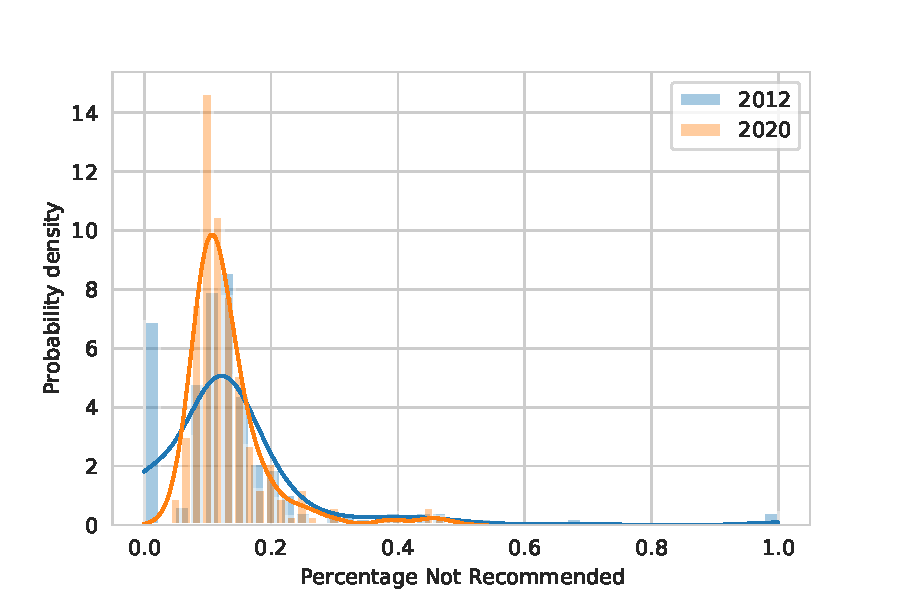
\includegraphics[width=0.9\columnwidth]{chapters/reviews/figures/filtered_proportion_density.pdf}
    \caption{Probability density of Not Recommended review percentage for a business, 2012 and 2020 data. Lines are the kernel density estimates.}
    \label{fig:filtered_density}
\end{figure}

\begin{figure}[t]
    \centering
    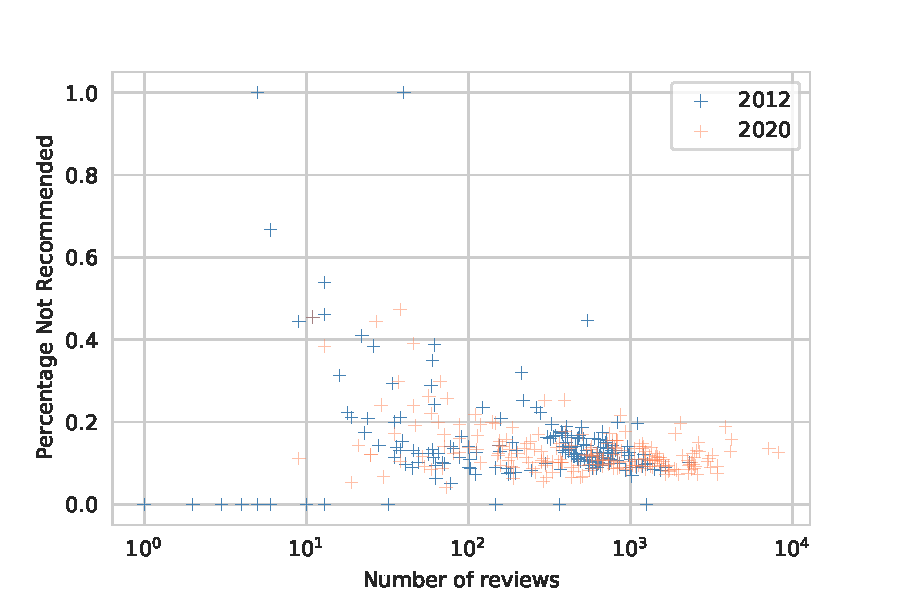
\includegraphics[width=0.9\columnwidth]{chapters/reviews/figures/filtered_vs_count.pdf}
    \caption{Number of reviews versus the percentage of reviews that were Not Recommended for a business, 2012 and 2020 data.}
    \label{fig:count_vs_perc}
\end{figure}

\textbf{The percentages of Not Recommended reviews by businesses tend to converge with more reviews.} To understand whether review classification has changed at a business level, we examined the distribution of percentage of Not Recommended reviews per businesses and the connection between number of reviews and percentage Not Recommended per business. Figure~\ref{fig:filtered_density} shows the distribution of percentage Not Recommended by business. The median percentage Not Recommended is similar (0.122 and 0.115), but the distributions are distinct (Kolmogorov–Smirnov test $\text{p}<0.01$). In the 2012, a number of business have no Not Recommended reviews. Some of these results may be explained by the business having fewer reviews in 2012 than 2020. Figure~\ref{fig:count_vs_perc} shows the connection between the number of reviews on a business and the percentage Not Recommended. Most businesses converge to around the same percentage Not Recommended with enough reviews. This convergence appears tighter among the 2020 data. We note that there is no significant correlation between the number of reviews and the percentage Recommended for the 2012 data (Spearman's correlation $\rho = 0.13$, $\text{p} = 0.06$), but there is a significant, negative correlation for the 2020 data ($\rho = -0.31$, $\text{p}<1\text{e}-5$)---the more reviews a business has, the smaller the proportion of Not Recommended reviews. The correlation for the 2020 data may be more significant because the businesses are more established.
%\rmNote{Suggested edit for above paragraph below. I tried to be a little more precise about the quantities at the cost of verbosity. Since the figures are plotted by Not Recommended reviews, I find that it's usually clearer to be consistent in the prose, especially since the semantics are equivalent. Also, I added paragraph structure to this subsection to make it clearer. If space concerns become acute, that paragraph structure can be recollapsed.}
% \textbf{The percentages of Not Recommended reviews by businesses tend to converge with more reviews.}
% To understand how reclassification has redistributed the classifications of Recommended and Not Recommended on reviews at the business level, we examine the distribution of the percentage of Not Recommended Reviews by business. We also examine the connection between the distribution of the number of reviews by business and the distribution of the percentage of those reviews that are Not Recommended.

%Figure~\ref{fig:filtered_density} shows the distributions of the percentage of Not Recommended Reviews by business observed in the two snapshots of the EYG dataset. Although the medians are similar (0.122 and 0.155 in the 2012 and 2020 snapshots, respectively), the distributions are distinct (Kolmogorov–Smirnov test $\text{p}<0.01$). In the 2012 snapshot, some businesses have zero Not Recommended reviews; this may be explained for at least some of these businesses by the observation that businesses generally had fewer reviews in 2012 than 2020.

%Figure~\ref{fig:count_vs_perc} shows the connection between the distribution of the number of reviews by business and the distribution of the percentage of those reviews that are Not Recommended in the EYG dataset. In both snapshots, it appears that the percentages of Not Recommended reviews by business converge with more reviews, and this convergence appears tighter in the 2020 snapshot. Although we observe no significant correlation between the number of reviews on a business and the percentage of those reviews that are Not Recommended in the 2012 snapshot (Spearman's correlation $\rho = 0.13$, $\text{p}>0.05$), there is a significant and negative correlation in the 2020 snapshot ($\rho = -0.31$, $\text{p}<1\text{e}-5$)---the more reviews a business has, the smaller the percentage of Not Recommended reviews is likely to be. The correlation observed in the 2020 snapshot may be more significant because the businesses are more established.

\begin{table}[t]
    \centering
    \caption{Frequency of reclassification patterns observed in Chicago data over 5 timepoints. ``R'' denotes Recommended, ``N'' denotes Not Recommended.}
    \label{tab:reclassification_patterns}
    \begin{tabular}{llr}
    \# changes & Pattern & Count \\
	 \hline
	 0 & R & 1,235,194\\
	 & N & 148,278\\
	 & \textit{Total} & 1,383,472 \\
	 \hline
	 1& R $\to$ N & 4,953\\
	 & N $\to$ R & 5,573\\
	 & \textit{Total} & 10,526\\
	 \hline
	 2& R $\to$ N $\to$ R & 706\\
	 & N $\to$ R $\to$ N & 373\\
	 & \textit{Total} & 1079\\
	 \hline
	 3+ & R $\to$ N $\to$ R $\to$ N & 60\\
	 & N $\to$ R $\to$ N $\to$ R & 75\\
	 & R $\to$ N $\to$ R $\to$ N $\to$ R & 14\\
	 & N $\to$ R $\to$ N $\to$ R $\to$ N & 15\\
	 & N $\to$ R $\to$ N $\to$ R $\to$ N $\to$ R & 2\\
	 & \textit{Total} & 157\\
	 \hline
    \end{tabular}
\end{table}

\textbf{Many reviews are reclassified, a few are reclassified frequently.} To investigate the frequency and scale of reclassification on shorter timescales we investigate reviews from the CHI dataset. Table \ref{tab:reclassification_patterns} shows how frequently reviews were reclassified. In our study period, around 0.8\% of reviews were reclassified. A small fraction of reviews undergo a substantial number of changes. This is especially interesting in light of the shorter study period and the limited number of time-points---a few reviews changed classes almost every measurement. These reviews may be cases that are particularly hard for Yelp to classify. 
%\raNote{Does this fit a markov-model pattern where we assume with x\% probability of reclassifying model?}
%\rmNote{Suggested edit for above paragraph below. I'll delimit the end of the suggestion.}
%\textbf{Many reviews are reclassified, a few are reclassified frequently.}
%To investigate the frequency and scale of reclassification on shorter timescales we examine the CHI dataset. Table \ref{tab:reclassification_patterns} shows how frequently reviews were reclassified. In our study period, we did not observe a change in the classification of most reviews, we did observe reclassification at least once on around 0.8\% of reviews, and multiple times on a small fraction of reviews. This is especially interesting in light of the shorter study period and the limited number of time-points---a few reviews were reclassified almost every measurement! These reviews may be cases that are particularly hard for Yelp to classify.

%\rmNote{End of suggested edit.}

\begin{figure}[t]
    \centering
    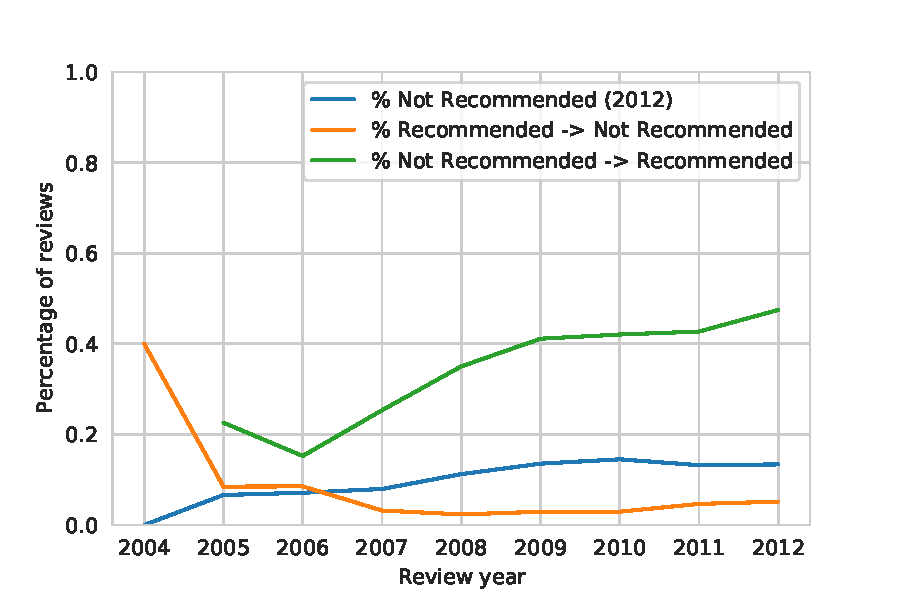
\includegraphics[width=0.9\columnwidth]{chapters/reviews/figures/filtering_changes.pdf}
    \caption{Change in recommendation status by the year reviews posted. The blue line represents reviews Not Recommended in 2012; the orange and green lines represent reviews that were Recommended and Not Recommended, respectively, in 2012 but reclassified in 2020. %\raNote{Would be good to change this to a CDF so it matches fig \ref{fig:reclassification_by_date_chicago}}
    }
    \label{fig:filtered_change}
\end{figure}

\textbf{In the long run, newer Not Recommended reviews are more likely to be reclassified.} To explore the relationship between reclassification and review age, we grouped reviews in EYG by the year posted. Within each group, we measured the percentage of reviews Yelp Recommended in 2012 and the percentage reclassified in 2020 from Recommended and Not Recommended (Figure \ref{fig:filtered_change}). Note that 2004 has just five reviews, and all were Recommended in 2012. The trend of the percentage Not Recommended in both 2012 and 2020 (green) suggests that Yelp was more likely to reclassify newer reviews from Not Recommended to Recommended. Yelp could have had more time to examine older reviews by 2012, or older, less sophisticated fake reviews may have resulted in fewer filtering errors to correct. Alternatively, this could stem from the use of review age or correlated factors (e.g., the number of reviews per author) in classification: Yelp considers whether a reviewer is ``established'' in recommending reviews~\cite{yelpwhyrec}.

\begin{figure}[t]
    \centering
    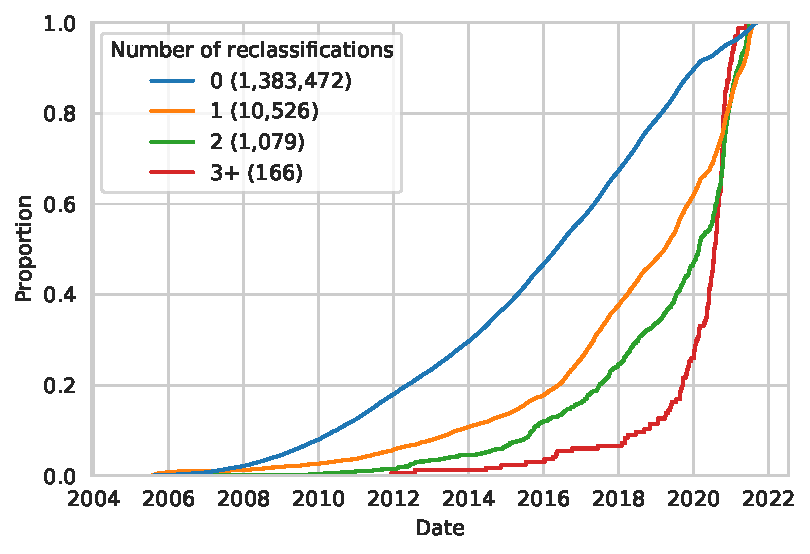
\includegraphics[width=0.9\columnwidth]{chapters/reviews/figures/reclassification_by_date_grouped_chicago.pdf}
    \caption{Cumulative percentage of reviews with a given number of reclassifications that were posted by a given date. For example, by the start of 2018 approximately 20\% of reviews with 2 observed reclassifications had been posted.}
    \label{fig:reclassification_by_date_chicago}
\end{figure}

\textbf{Newer reviews are more likely to undergo repeated reclassification, but the chance of reclassification persists over time.} Figure \ref{fig:reclassification_by_date_chicago}, shows reviews which undergo more frequent reclassification tend to be newer. This supports the idea that Yelp increases its confidence in classifying reviews as the reviews age. Perhaps because Yelp has observed more activity from the author's account or the business. We note that we still see reclassifications of reviews dating back to 2005, suggesting that a review's classification is never fully stable.
%We also see that there is little difference between the age of reviews that were reclassified zero or one times. This suggests that Yelp never fully stabilizes its classes -- even old reviews can have their classification revised.
We note a small artifact in the upper-right corner: the 1, 2, and 3+ lines rise above the 0 line. We expect this artifact because the newest reviews cannot have 1, 2, or 3+ reclassifications, since we have not made as many observations of them. These results support Yelp's statement that their classifier may mark a review as Not Recommended if it does not have sufficient data to recommend it \cite{yelprecommendationsoftware}.

Given these results showing that newer reviews are more likely to undergo reclassification and the disparity between the percentage reclassified for the EYG (8.69\% over 8 years) and CHI datasets (0.87\% over 11 months), it seems likely that Yelp's classifer is either more stable today or that Yelp performed a major overhaul between the EYG collection time-points. It's also possible that the EYG sample was disproportionately subject to reclassification.

%\raNote{I guess we could actually test this with CHI...}

% \begin{figure}[t]
%     \centering
%     \includegraphics[width=0.9\columnwidth]{figures/author_based_recommended_matching.pdf}
%     \caption{The distribution of the percentage of an author's other reviews that match the class of a given review. Reviews come from authors with two or more reviews. \raNote{Maybe there's a better way to present this. Also show reclassification instead}}
%     \label{fig:author_based_recommended_matching}
% \end{figure}

\textbf{Review classes follow the author.} In order to determine if reclassifications are performed at the author level, we investigated whether authors who have a review classifcation change are likely to have their other reviews match the new classification. In the 1,175 cases in which an author with multiple reviews had a review reclassified, 924 had all of their reviews match after reclassification. The average percentage of an author's review pairs that matched classification was 95.1\% for Recommended reviews and 94.7\% for Not Recommended reviews. This suggests that classifications follow the author.

%\raNote{ideally more analysis?}

We did not find that any particular timepoint had significantly more reclassifications.

% \raNote{maybe we can put some of the other null results here?}



% \begin{figure}[t]
%     \centering
%     \includegraphics[width=0.9\columnwidth]{figures/}
%     \caption{}
%     \label{fig:}
% \end{figure}

%Make this into a table and use constants

%0            1,305,376
%1            18,865
%2            463
%3            23
%4            1

%Non-duplicated        1324728
%Duplicated        1593

%+        1176516
%-         142541
%-+          3078
%+-          2139
%+-+          253
%-+-          177
%-+-+          15
%+-+-           8
%-+-+-          1


\subsection{Density and income impacts}

We were investigated how density and income impact reviews using our UDIS study.



\begin{figure}[t]
    \centering
    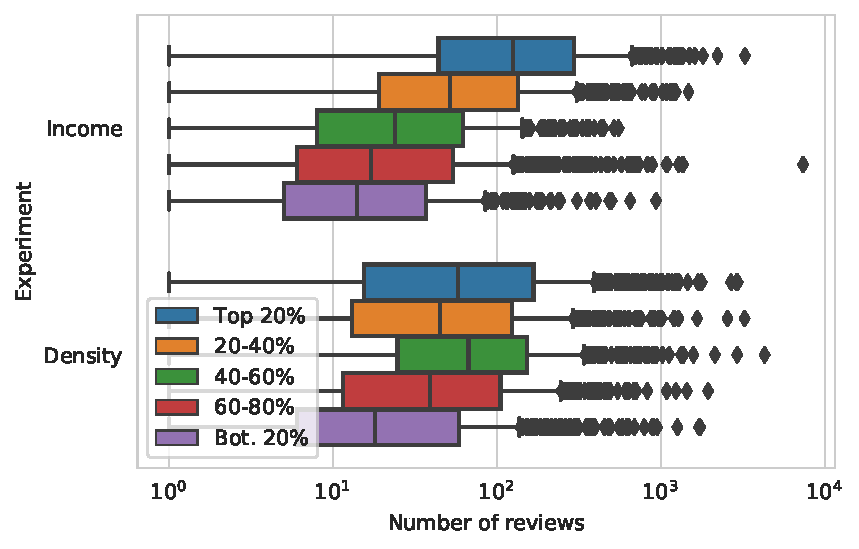
\includegraphics[width=0.9\columnwidth]{chapters/reviews/figures/reviews_per_business_stratified.pdf}
    \caption{Reviews per business. Each data point is the number of reviews for one business. }
    \label{fig:reviews_per_business_stratified}
\end{figure}

\textbf{Demographic factors correlate with the number of reviews on each business.} We investigated the number of reviews per business in Figure \ref{fig:reviews_per_business_stratified}. Both low income and low density areas have fewer reviews per business than higher income and higher density areas, and the gap is wider for density. This could be because higher income areas typically have businesses with more time on the platform---for the highest income stratum the median oldest review for each business (3,425 days) is 30\% older than for the lowest income stratum (2,638 days). This relationship is not as strong in the density experiment: the middle density stratum has the oldest reviews (3,245 days), slightly higher than the highest stratum (3,066 days) and much higher than the lowest stratum (2,704 days). The disparity in number of reviews means consumers in these areas may have less access to reviews, impacting their ability to make good decisions.

 \begin{figure}[t]
     \centering
     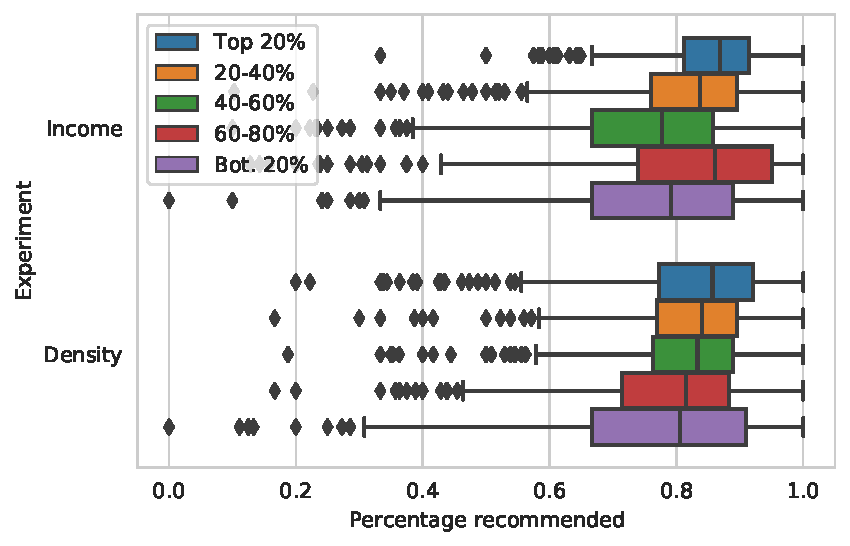
\includegraphics[width=0.9\columnwidth]{chapters/reviews/figures/percentage_recommended_per_businesses_extended.pdf}
     \caption{The proportion of reviews Recommended per business. Each data point represents one business.}
     \label{fig:percentage_recommended_per_businesses_extended}
 \end{figure}
 
\textbf{Demographic factors correlate with the percentage of reviews Recommended for each business.} We examined how the percentage of reviews that are Recommended per business varies by income and density in Figure \ref{fig:percentage_recommended_per_businesses_extended}. The range in median percentage Recommended is tighter for density---it ranges from 80\% (Bottom 20\%) to 86\% (Top 20\%)---whereas the range is larger for income, ranging from 78\% (40-60\%) to 87\% (Top 20\%). 

\begin{figure}[t]
    \centering
    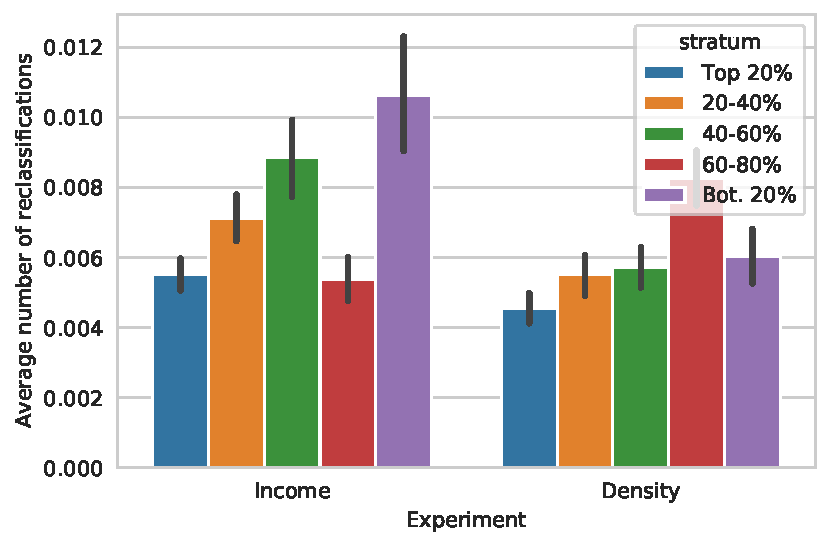
\includegraphics[width=0.9\columnwidth]{chapters/reviews/figures/stratified_reclass_swaps_usa.pdf}
    \caption{Average number of reclassifications per unique review per stratrum. Black bars indicate the 95\% confidence interval}
    \label{fig:stratified_reclass_swaps_usa}
\end{figure}

\textbf{Demographic factors correlate with the frequency of reclassifications.} In Section \ref{subsec:review_reclassification}, we explored the frequency and factors surrounding reclassification. To test whether Yelp reclassifies reviews for businesses in regions with certain income or density attributes more frequently, we looked at the average number of reclassifications per review in each stratum for both the UIS and UDS crawls (Figure \ref{fig:stratified_reclass_swaps_usa}). Less dense and lower income regions experience more reclassification. The 60-80\% strata are an outlier in both cases---the 60-80\% density stratum experiences significantly more reclassifications while the 60-80\% income stratum experiences significantly less than its neighbors, but on par with the top income stratum, which warrants further research. These disparities invite questions as to why they arise: is there something inherent about these markets that leads to more challenging-to-classify reviews, or is Yelp's classifier not well tuned to them?



\subsection{Masking}

\begin{figure}[t]
    \centering
    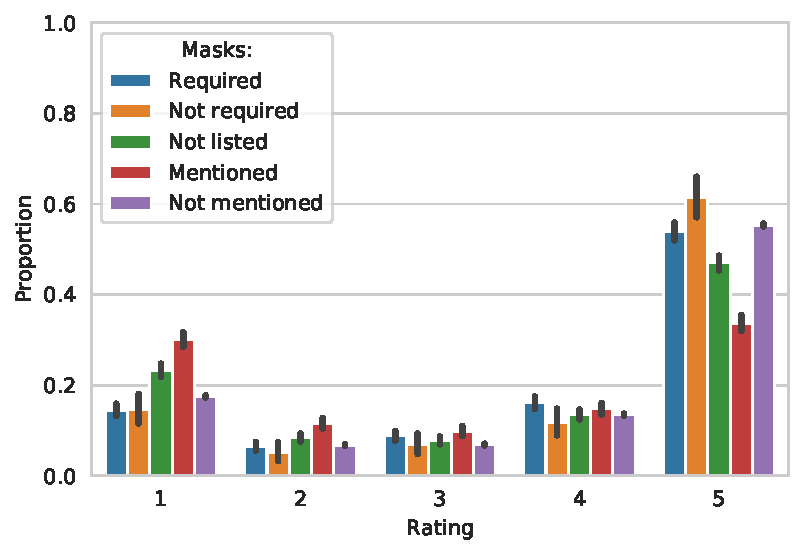
\includegraphics[width=0.9\columnwidth]{chapters/reviews/figures/proprotion_Masks_by_Rating_usa.pdf}
    \caption{The proportion by rating of reviews on or after August 06, 2021 on businesses that require/do not require/do not list a requirement for masks and reviews on or after March 1, 2020 that mention/do not mention masks. Black bars indicate the 95\% confidence interval.
    %\raNote{Update -- change order, clean up labels, y axis label}
    }
    \label{fig:proprotion_Masks mentions_masks required_by_rating_usa}
\end{figure}

In response to the COVID-19 pandemic, Yelp added an option for businesses to specify a mask policy in August 2021. Because this coincided with our longitudinal data collection, we studied reviews that mention masks and business with listed mask policies. We used our UDIS-4 crawl data because that crawl started after Yelp added the option. 

We determined whether a review mentioned masks by tokenizing the review and lemmatizing the tokens. If any lemma matched ``mask", we considered that review to mention masks. We find that 90.2\% (2,845) of UDIS reviews mentioning masks occur on or after March 1, 2020. We manually examined a random sample of 20 such reviews from before March 1, 2020; 16 of used ``mask'' to describe covering a taste or odor, 1 in a COVID-19 context, and 3 to describe costumes. We examined a random sample of 20 such reviews from on or after March 1, 2020; all 20 of them used ``mask'' in a COVID-19 context. To determine whether a business has a masking policy, we used the business amenities as described in Section \ref{subsec:crawling}. We found 837 businesses requiring masks, 174 not requiring masks, and 4,666 with no listed policy.

\textbf{Mask policies have little correlation with rating, as long as one is present. Discussions of masks correspond to lower ratings.} We show how both customer mask requirements and mask discussion affect rating in Figure \ref{fig:proprotion_Masks mentions_masks required_by_rating_usa}. Reviews mentioning masks have a lower rating, and this relationship remains after removing Not Recommended reviews. Having a mask requirement results in a slightly lower rating (means 3.89 and 4.00, Spearman correlation $\rho = -0.04$, $\text{p}<0.05$), but this relationship vanishes after removing Not Recommended reviews (mean 3.92 and 3.90, Spearman correlation $\rho = -0.01$, $\text{p}=0.79$). This suggests Yelp's filter may have the effect of protecting restaurants requiring masks. Listing any policy correlates with higher ratings; this could be explained by the overall correlation between higher ratings and more listed amenities: the Spearman's rank correlation between the rating and the number of amenities is $\rho=0.119$ $(\text{p}<<1\text{e}-5)$.   % \raNote{scipy says p=0 but that must be floating point rounding}.




\section{Discussion} \label{sec:rim:discussion}
Online reviews are part of an actively evolving landscape with significant economic consequences. In this paper, we have examined this landscape from four different cross-sections: a course-grained eight year view;
a more fine-grained, eleven month view focused on one region; a four month view sampled from the whole US stratified by density; and a second four month view stratified by income. Each of these datasets is available for other researchers to use.

Reviews on Yelp routinely move between classifications, in both directions, occasionally multiple times. Newer reviews are less stable in their classification, but even old reviews are still subject to occasional reclassification, even multiple reclassifications. These reclassifications are often connected to the review author. Density and income are connected to the number of reviews per business and how frequently reviews are reclassified. Finally, both discussion of masks and, to a lesser extent, declaring a mask policy, impact the ratings given by reviewers.

Our results have implications for platforms and regulators. Our reclassification results demonstrate the uncertainty in the recommendation process. This calls for transparency on the part of the platform; Yelp's policy of making Not Recommended reviews available helps here. Furthermore, platforms should be cautious about changing classification until they are confident the review is not problematic. 
%\pmNote{what are the recommendations based on our reclassification analysis in coarse/fine data crawls?}
Platforms and regulators should consider carefully any discrepancies by density and income: are there steps that can be taken to address these inequities? Our observations surrounding masking policies suggest public backlash against a mask policy decision is negligible, which may be due in part to Yelp's classifier.


\subsection{Limitations} \label{subsec:rim:limitations}
%\raNote{Make this more delicate}

Our study is limited to a single platform and a single country, so it may not be representative of trends on other platforms or other countries. Our study period includes the COVID-19 pandemic, a period of substantial social and economic disruption~\cite{altig2020economic,deb2020economic}. Furthermore, local median income and population density may not completely describe the businesses and reviewers; for example reviewers may travel from another area to the business or the area may be heterogeneous.

%There is also some variation in the spacing between crawls, with the separation between crawl starts ranging from 1 month to 2.5 months. 
%\pmNote{why is this variation a limitation? maybe rephrase to say that the granularity of our crawls is approximately on the order of a month, and that we may have missed reclassifications in between etc. But this would make our analysis *conservative*, so would be good to mention that}

We expect that we may have missed reclassifications that occurred between crawl points and our crawler may have missed reviews (e.g. if the reviews reordered mid-crawl due to a new review). This means that some reviews may have been reclassified more frequently than we observed.
%\pmNote{does our analysis require completeness? if we don't make any claims about completeness, consider omitting this to simplify the discussion}

We also do not have a complete view of the review space---we have limited information on reviews removed for terms of service violations and no information on reviews removed by their author before our first crawl. Some of these reviews may be reviews of interest---for example, some problematic reviews may be removed entirely instead of made Not Recommended. %\pmNote{why is ToS violation removal important for our analysis? if some reviews were removed before our crawl, what is the impact on the analysis? If not important, consider removing the limitation}

% Our quality checks should help mitigate this concern.
%\pmNote{this is a very important point: a reviewer may bring this up when looking at the crawling methodology too. Why don't we random sample some reviews manually to see if content/filtering decision is a match? and if we did, we should mention this as a validation in the crawling section and skip mentioning it as a limitation}
%\pmNote{important: if we list this limitation, then lets briefly remind the reader of the validation step again here.}
\section{Collected data} \label{apd:collection}

\begin{table}[h!]
    \centering
    \caption{Data and metadata collected.}% \raNote{Numbers may be slightly off -- double check}}
    \label{tab:data_collected}
    \resizebox{\columnwidth}{!}{
    \begin{tabular}{l|l}
		  \toprule
            Field & Description \\
			\midrule
			Reviews\\
			\midrule
			Content & Text of the review\\
			Author ID & Identifier is different for Recommended and not Recommend reviews\\
			Date & Date of posting\\
			Rating & Review rating \\
			Business ID & Identifier for the business the review was posted to\\
			Author data & Name and other public account information\\
			Recommended & Whether the review is Recommended\\
			\midrule
			Businesses\\
			\midrule
			Business ID & Identifier for the business\\
			Amenities & Listed amenities\\
			\bottomrule
    \end{tabular}
    }
\end{table}

\begin{figure}[h!]
    \centering
    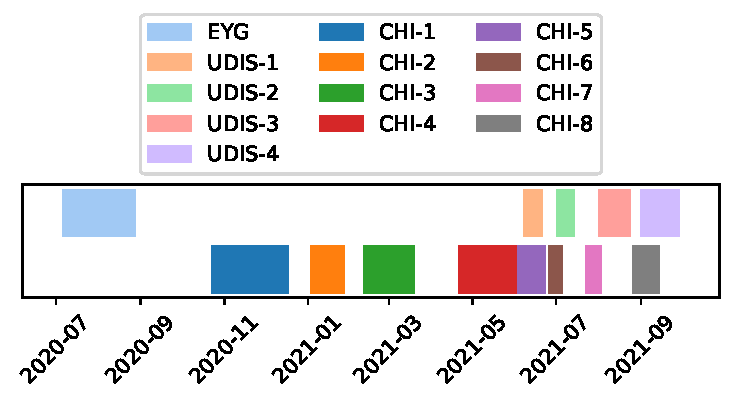
\includegraphics[width=0.9\columnwidth]{chapters/reviews/figures/crawl_timeline.pdf}
    \caption{The timeline for each crawl. Each box indicates the first and last operation for each crawl.}
    \label{fig:crawl_timeline}
\end{figure}

\begin{figure}[b!]
    \centering
    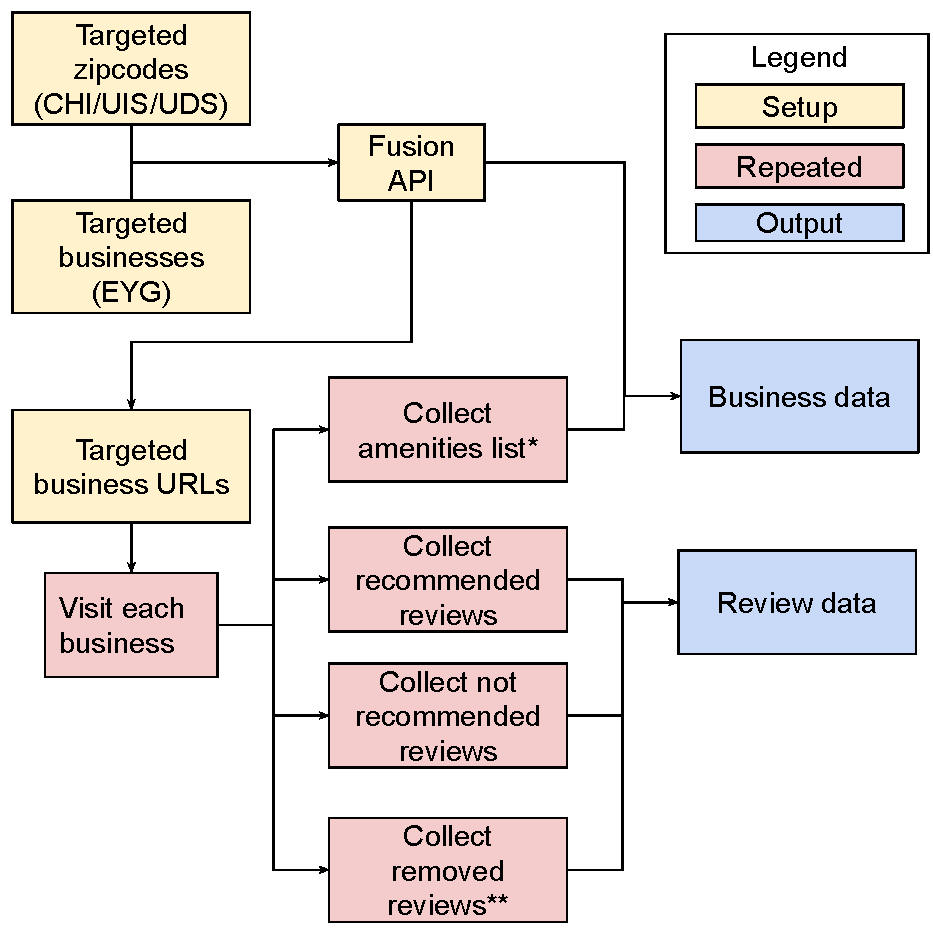
\includegraphics[width=0.9\columnwidth]{chapters/reviews/figures/Crawl diagram.pdf}
    \caption{The data collection process. Yellow indicates setup steps that are completed once. Red indicates steps that are completed for each timepoint. Blue indicates outputs.\\
    * Amenities were only collected for the CHI 8 and UDIS 4.\\
    ** Removed reviews were collected for CHI 7-8 and UDIS 3-4. }
    \label{fig:crawling_diagram}
\end{figure}

Lessons, takeaways, impact

Future work

Brief summary

% Make the bibliography single spaced
\singlespacing
\bibliographystyle{plainnat}

% add the Bibliography to the Table of Contents
\cleardoublepage
\ifdefined\phantomsection
  \phantomsection  % makes hyperref recognize this section properly for pdf link
\else
\fi
\addcontentsline{toc}{chapter}{Bibliography}

% include your .bib file
\bibliography{ref}

\appendix % all chapters following will be labeled as appendices
\doublespacing
% \include{ch-appendicies/simulation}
% \include{ch-appendicies/external}
%\include{ch-appendicies/suppl-figs-jointInference}
%\include{ch-appendicies/suppl-figs-ifaceMapping}

\end{document}

